\chapter[Resultados]{Resultados}

% palavras chaves para pesquisa
%PROJETO ASEPRITE TABELAS 

\section{Aplicado no Ambiente}

\begin{itemize}
    \item Tabelas e Gráficos
\end{itemize}

\begin{table}[!ht]
\centering
\caption{Resultados Guardas de Inclusão aplicado no Linux}
\label{tab:resutados_guards_de_inclusao:linux}
\begin{tiny}
\begin{tabular}{lp{1cm}p{1cm}p{1cm}p{1cm}p{1cm}p{1cm}p{1cm}p{1cm}}
\textbf{Tipo} & \multicolumn{7}{l}{Utilização de Guarda de Inclusão} \\
\textbf{Medida} & \multicolumn{7}{l}{Tempos em segundos } \\
\textbf{Amostras} & \textbf{GIE} & \textbf{GII} & \textbf{PO} & 
\textbf{GIIPPO} & \textbf{POPGII} & \textbf{GIEPO} & \textbf{RGI} \\ \toprule
 1      & 1.8942     & 0.3631  & 1.2690    & 1.3759    & 1.2709  & 1.2828     & 0.1909 \\
 2      & 0.3203     & 0.2732  & 1.2041    & 1.3253    & 1.2378  & 1.2307     & 0.1597 \\
 3      & 0.2939     & 0.2691  & 1.2109    & 1.3102    & 1.2394  & 1.2417     & 0.1593 \\
 4      & 0.2771     & 0.2784  & 1.1840    & 1.3350    & 1.2084  & 1.2215     & 0.1581 \\
 5      & 0.2814     & 0.2752  & 1.1681    & 1.3127    & 1.2051  & 1.2428     & 0.1557 \\
 6      & 0.2817     & 0.2771  & 1.2051    & 1.3036    & 1.2358  & 1.2452     & 0.1592 \\
 7      & 0.2838     & 0.2791  & 1.2311    & 1.2976    & 1.2503  & 1.2388     & 0.1565 \\
 8      & 0.2846     & 0.2729  & 1.2077    & 1.3105    & 1.2225  & 1.2404     & 0.1559 \\
 9      & 0.2970     & 0.2797  & 1.2058    & 1.2948    & 1.2335  & 1.2658     & 0.1584  \\
 10     & 0.3108     & 0.2829  & 1.2408    & 1.3124    & 1.2077  & 1.2679     & 0.1575  \\ \bottomrule
 Média: & 0.2851     & 0.2851  & 1.2127    & 1.3179    & 1.2311  & 1.2477     & 0.1611 \\
\end{tabular}
\end{tiny}
\end{table}

\begin{table}[!ht]
\centering
\caption{Resultados Guardas de Inclusão aplicado no Mac OS Yosemite}
\label{tab:resutados_guards_de_inclusao:mac}
\begin{tiny}
\begin{tabular}{lp{1cm}p{1cm}p{1cm}p{1cm}p{1cm}p{1cm}p{1cm}p{1cm}}
\textbf{Tipo} & \multicolumn{7}{l}{Utilização de Guarda de Inclusão} \\
\textbf{Medida} & \multicolumn{7}{l}{Tempos em segundos } \\
\textbf{Amostras} & \textbf{GIE} & \textbf{GII} & \textbf{PO} & 
\textbf{GIIPPO} & \textbf{POPGII} & \textbf{GIEPO} & \textbf{RGI} \\ \toprule
 1      & 0.8753 & 0.8249 & 1.0309  & 0.8424  & 0.7564  & 0.9224  & 0.6065  \\ 
 2      & 0.8422 & 0.8275 & 0.7369  & 0.7748  & 0.7616  & 0.8796  & 0.5017  \\ 
 3      & 0.7950 & 0.8539 & 0.9389  & 0.8111  & 0.7928  & 0.8366  & 0.5277  \\ 
 4      & 0.7599 & 0.7930 & 1.1065  & 0.9166  & 0.7444  & 0.8158  & 0.5033  \\ 
 5      & 0.8539 & 0.7760 & 0.8515  & 1.0654  & 0.8573  & 0.7830  & 0.5114  \\ 
 6      & 0.9596 & 0.8868 & 1.0004  & 0.9729  & 1.3346  & 0.8005  & 0.5864  \\ 
 7      & 0.8569 & 0.8558 & 1.0348  & 1.3181  & 1.2343  & 0.8366  & 0.5791  \\ 
 8      & 0.7840 & 0.7600 & 1.0462  & 1.2104  & 1.2177  & 0.9315  & 0.5044  \\ 
 9      & 0.7987 & 0.8231 & 1.1556  & 1.2441  & 0.9490  & 1.2485  & 0.7518  \\ 
 10     & 0.9568 & 0.7484 & 1.1298  & 0.9836  & 0.8628  & 1.0419  & 0.5954  \\ \bottomrule
 Média: & 0.8482 & 0.8149 & 1.0031  & 1.0139  & 0.9511  & 0.9097  & 0.5668  \\ 
\end{tabular}
\end{tiny}
\end{table}

\begin{table}[!ht]
\centering
\caption{Resultados Guardas de Inclusão aplicado no Windows 7}
\label{tab:resutados_guards_de_inclusao:windows7}
\begin{tiny}
\begin{tabular}{lp{1cm}p{1cm}p{1cm}p{1cm}p{1cm}p{1cm}p{1cm}p{1cm}}
\textbf{Tipo} & \multicolumn{7}{l}{Utilização de Guarda de Inclusão} \\
\textbf{Medida} & \multicolumn{7}{l}{Tempos em segundos } \\
\textbf{Amostras} & \textbf{GIE} & \textbf{GII} & \textbf{PO} & 
\textbf{GIIPPO} & \textbf{POPGII} & \textbf{GIEPO} & \textbf{RGI} \\ \toprule
 1      & 2.4736 & 2.4535 & 4.2161 & 4.4164 & 4.3262 & 4.3863  & 2.1030 \\ 
 2      & 2.3634 & 2.3834 & 4.1760 & 4.3162 & 4.3062 & 4.2761  & 2.1030 \\ 
 3      & 2.4235 & 2.4135 & 4.2962 & 4.2060 & 4.2962 & 4.2261  & 2.1331 \\ 
 4      & 2.4035 & 2.3934 & 4.4564 & 4.2962 & 4.3563 & 4.2060  & 2.1531 \\ 
 5      & 2.3634 & 2.3534 & 4.2161 & 4.2661 & 4.2962 & 4.3663  & 2.1130 \\ 
 6      & 2.3834 & 2.3634 & 4.1560 & 4.2561 & 4.2862 & 4.2461  & 2.1030 \\ 
 7      & 2.4235 & 2.3734 & 4.1660 & 4.2161 & 4.3262 & 4.1960  & 2.2032 \\ 
 8      & 2.4035 & 2.4235 & 4.1460 & 4.2060 & 4.3663 & 4.2261  & 2.2933 \\ 
 9      & 2.3934 & 2.4235 & 4.1760 & 4.2261 & 4.2862 & 4.2561  & 2.1331 \\ 
 10     & 2.3834 & 2.3734 & 4.1560 & 4.2060 & 4.3062 & 4.2361  & 2.1331 \\ \bottomrule 
 Média: & 2.4015 & 2.3954 & 4.2161 & 4.2611 & 4.3152 & 4.2621  & 2.1471 \\
\end{tabular}
\end{tiny}
\end{table}

\begin{figure}[!h]
    \centering
        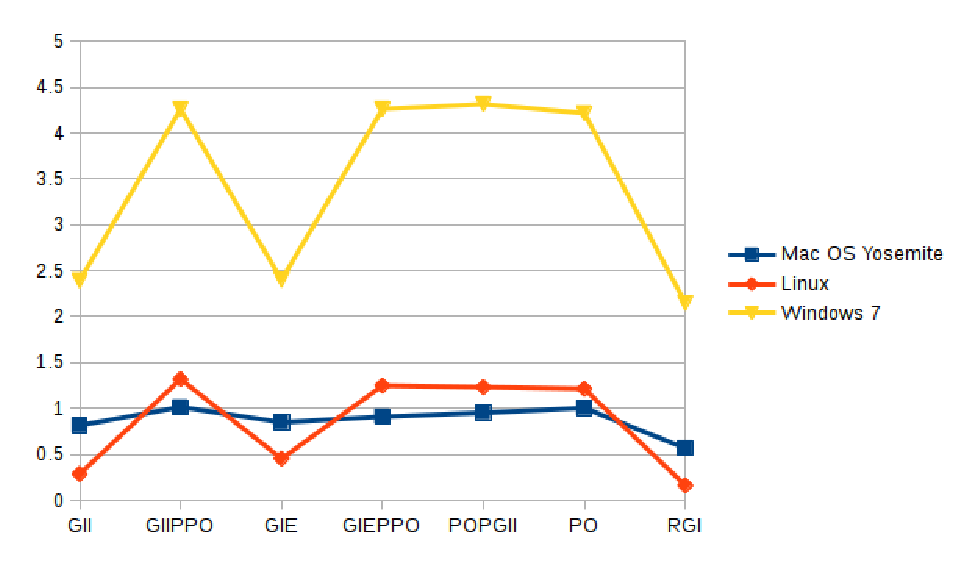
\includegraphics{figuras/graficos/benchmark.eps}
    \caption{Dados coletados dos scripts de Guardas de Inclusão}
    \label{benchmark_guardas_de_inclusao}
\end{figure}

\begin{itemize}
     \item Analise

    Com base nos dados coletados e o gráfico gerado é possível concluir :
    \begin{enumerate}
        \item Todos os métodos que incluem \texttt{pragma once} atigiram tempo de compilação maior que os métodos que não possuem, independente do sistema operacional;
        \item Dos métodos que não possuem \texttt{\#pragma once} o método redundante foi o que atingiu o menor tempo de compilação;
        \item Em sistema operacional Mac OS Yosemite o tempo de compilação entre os métodos possui a menor variação.
        \item Em ambiente Windows 7 o tempo de compilação dos métodos é entre 3 e 4 vezes maior que nos outros sistemas operacionais. 
    \end{enumerate}
\end{itemize}

\clearpage
\section{Aplicado no Projeto}

\subsection{Alteração no Código}\label{resultados_alteracao_de_codigo}

\begin{itemize}
    \item Tabelas e Gráficos

\end{itemize}

\subsubsection*{Aseprite}
%  PROJETO ASEPRITE TABELAS

\begin{table}[!h]
\tiny
\centering
\caption{Aseprite - Alteração de Código no Linux }
\label{tab:alteracao_de_codigo:linux:aseprite}
\begin{tabular}{lllll}
\textbf{Aseprite} & \textbf{master} & \textbf{pragma once} & \textbf{forward declaration} & \textbf{private implementation}   \\ \toprule
1                      &    2514.9207         &  2418.7051   &  -   &  -   \\ 
2                      &    2333.7905         &  2370.1243   &  -   &  -   \\ 
3                      &    2352.6054         &  2358.9848   &  -   &  -   \\ 
4                      &    2341.8494         &  2346.8402   &  -   &  -   \\ 
5                      &    2326.8056         &  2347.7365   &  -   &  -   \\ 
6                      &    2342.5205         &  2367.7181   &  -   &  -   \\ 
7                      &    2339.0471         &  2347.5773   &  -   &  -   \\ 
8                      &    2335.0176         &  2364.5381   &  -   &  -   \\ 
9                      &    2344.1943         &  2352.7533   &  -   &  -   \\ 
10                     &    2347.9277         &  2351.9232   &  -   &  -   \\ \bottomrule
Média                  &    2357.8679         &  2362.6901   &  -   &  -   \\ 
\end{tabular}
\end{table}

\begin{table}[!h]
\tiny
\centering
\caption{Aseprite - Alteração de Código no Mac OS Yosemite }
\label{tab:alteracao_de_codigo:mac:aseprite}
\begin{tabular}{lllll}
\textbf{Aseprite} & \textbf{master} & \textbf{pragma once} & \textbf{forward declaration} & \textbf{private implementation}   \\ \toprule
1                       & 788.2866           &793.1793 &  -   &  -   \\ 
2                       & 767.4185           &778.4403 &  -   &  -   \\ 
3                       & 764.6951           &769.6590 &  -   &  -   \\ 
4                       & 764.9236           &772.5233 &  -   &  -   \\ 
5                       & 779.1553           &771.1125 &  -   &  -   \\ 
6                       & 763.0460           &767.2010 &  -   &  -   \\ 
7                       & 764.7422           &768.7916 &  -   &  -   \\ 
8                       & 768.9518           &768.6012 &  -   &  -   \\ 
9                       & 764.8288           &765.9876 &  -   &  -   \\ 
10                      & 765.5380           &769.1677 &  -   &  -   \\ \bottomrule
Média                   & 769.1586           &772.4663 &  -   &  -   \\ 
\end{tabular}
\end{table}

\begin{table}[!h]
\tiny
\centering
\caption{Aseprite - Alteração de Código no Windows 7}
\label{tab:alteracao_de_codigo:windows:aseprite}
\begin{tabular}{lllll}
\textbf{Aseprite} & \textbf{master}  & \textbf{pragma once} & \textbf{forward declaration} & \textbf{private implementation}   \\ \toprule
1                     &    2504.0313          & 2348.2715  &  -   &  -   \\ 
2                     &    2462.2656          & 2320.0910  &  -   &  -   \\ 
3                     &    2429.9063          & 2316.0552  &  -   &  -   \\ 
4                     &    2419.6250          & 2322.7848  &  -   &  -   \\ 
5                     &    2436.5938          & 2313.0809  &  -   &  -   \\ 
6                     &    2413.1406          & 2311.7142  &  -   &  -   \\ 
7                     &    2444.6719          & 2310.8516  &  -   &  -   \\ 
8                     &    2437.4375          & 2310.6613  &  -   &  -   \\ 
9                     &    2437.3125          & 2307.9774  &  -   &  -   \\ 
10                    &    2428.8438          & 2310.4009  &  -   &  -   \\ \bottomrule
Média                 &    2441.3828          & 2317.1889  &  -   &  -   \\ 
\end{tabular}
\end{table}


\clearpage
%  PROJETO IRECOVERYPLUSPLUS TABELAS
\subsubsection*{iRecoveryplusplus}

\begin{table}[!h]
\centering
\tiny
\caption{iRecoveryplusplus - Alteração de Código no Linux}
\label{tab:alteracao_de_codigo:linux:irecovery}
\begin{tabular}{lllll}
\textbf{iRecoveryplusplus} & \textbf{master}   & \textbf{pragma once} & \textbf{forward declaration} & \textbf{private implementation}   \\ \toprule
1                     &   1.1434           & 0.8880   & 1.0075   &  0.8692     \\ 
2                     &   1.0827           & 0.8912   & 0.9056   &  0.8717     \\ 
3                     &   1.1257           & 0.8359   & 0.8436   &  0.9154     \\ 
4                     &   1.0751           & 0.8506   & 0.8626   &  0.8796     \\ 
5                     &   1.0623           & 0.8314   & 0.9103   &  0.8760     \\ 
6                     &   1.1633           & 0.8658   & 0.8285   &  0.8405     \\ 
7                     &   1.0963           & 0.8921   & 0.9060   &  0.9267     \\ 
8                     &   1.4273           & 0.7975   & 0.9121   &  1.0221     \\ 
9                     &   1.0871           & 0.8991   & 0.8943   &  0.9513     \\ 
10                    &   1.4181           & 0.8476   & 0.9039   &  0.9898     \\ \bottomrule
Média                 &   1.1681           & 0.8599   & 0.8975   &  0.9142     \\ 
\end{tabular}
\end{table}

\begin{table}[!h]
\tiny
\centering
\caption{iRecoveryplusplus - Alteração de Código no Mac OS Yosemite}
\label{tab:alteracao_de_codigo:mac:irecovery}
\begin{tabular}{lllll}
\textbf{iRecoveryplusplus} & \textbf{master}  & \textbf{pragma once} & \textbf{forward declaration} & \textbf{private implementation}   \\ \toprule
1                   &  2.7747              & 2.7420 & 2.6686 & 2.6628 \\ 
2                   &  2.9096              & 2.6853 & 2.6563 & 2.5578 \\ 
3                   &  2.8155              & 2.6057 & 2.7956 & 2.7908 \\ 
4                   &  2.8629              & 2.8325 & 2.6673 & 2.7269 \\ 
5                   &  2.8847              & 2.8229 & 2.7536 & 2.7051 \\ 
6                   &  2.8877              & 3.0290 & 2.7412 & 2.6424 \\ 
7                   &  2.8877              & 3.1176 & 2.6894 & 2.6555 \\ 
8                   &  2.8634              & 3.1709 & 2.6639 & 2.8007 \\ 
9                   &  2.7734              & 3.1759 & 2.6337 & 2.6727 \\ 
10                  &  2.8015              & 3.0473 & 2.6510 & 2.7748 \\ \bottomrule
Média               &  2.8461              & 2.9229 & 2.6921 & 2.6990 \\ 
\end{tabular}
\end{table}

\begin{table}[!h]
\tiny
\centering
\caption{iRecoveryplusplus - Alteração de Código no Windows 7}
\label{tab:alteracao_de_codigo:windows:irecovery}
\begin{tabular}{lllll}
\textbf{iRecoveryplusplus} &  \textbf{master}  & \textbf{pragma once} & \textbf{forward declaration} & \textbf{private implementation}   \\ \toprule
1                            &  4.4375     & 5.0447  & 4.2836  & 4.8445 \\ 
2                            &  4.7969     & 4.9847  & 4.2937  & 4.8344 \\ 
3                            &  4.7969     & 4.9947  & 4.3037  & 4.8344 \\ 
4                            &  4.8438     & 5.0047  & 4.2836  & 4.7944 \\ 
5                            &  5.1094     & 4.9847  & 4.2536  & 4.8344 \\ 
6                            &  5.6875     & 4.9947  & 4.3437  & 4.8344 \\ 
7                            &  5.0625     & 5.0347  & 4.2836  & 4.8244 \\ 
8                            &  5.1719     & 5.0648  & 4.3437  & 4.8545 \\ 
9                            &  5.0156     & 5.0447  & 4.3037  & 4.8545 \\ 
10                           &  4.7656     & 5.0347  & 4.3037  & 4.8244 \\ \bottomrule
Média                        &  4.9688     & 5.0187  & 4.2997  & 4.8334 \\ 
\end{tabular}
\end{table}

\clearpage
%  PROJETO PENCIL TABELAS
\subsubsection*{Pencil}

\begin{table}[!h]
\tiny
\centering
\caption{Pencil - Alteração de Código no Linux}
\label{tab:alteracao_de_codigo:linux:pencil}
\begin{tabular}{lllll}
\textbf{Pencil} & \textbf{master} & \textbf{pragma once} & \textbf{forward declaration} & \textbf{private implementation}   \\ \toprule
1                        &   455.6515         &  459.8221  &  -   & 455.7540      \\ 
2                        &   458.6480         &  457.9709  &  -   & 453.2132      \\ 
3                        &   453.9845         &  458.2263  &  -   & 455.5010      \\ 
4                        &   452.3321         &  458.2057  &  -   & 454.1596      \\ 
5                        &   456.3933         &  456.9206  &  -   & 451.7834      \\ 
6                        &   452.3841         &  458.6638  &  -   & 451.9862      \\ 
7                        &   455.8518         &  461.7113  &  -   & 454.3775      \\ 
8                        &   454.1806         &  461.1395  &  -   & 453.9680      \\ 
9                        &   455.4113         &  456.5944  &  -   & 454.3351      \\ 
10                       &   455.8023         &  463.0633  &  -   & 453.5500      \\ \bottomrule 
Média                    &   455.0640         &  459.2318  &  -   & 453.8628      \\
\end{tabular}
\end{table}

\begin{table}[!h]
\tiny
\centering
\caption{Pencil - Alteração de Código no Mac OS Yosemite}
\label{tab:alteracao_de_codigo:mac:pencil}
\begin{tabular}{lllll}
\textbf{Pencil} & \textbf{master} & \textbf{pragma once} & \textbf{forward declaration} & \textbf{private implementation}   \\ \toprule
1                         &  355.0881         & 345.0807  &  -   & 355.7133  \\ 
2                         &  352.3484         & 345.0180  &  -   & 354.2093  \\ 
3                         &  353.0415         & 346.0400  &  -   & 352.3386  \\ 
4                         &  352.9057         & 344.8880  &  -   & 352.3613  \\ 
5                         &  352.1713         & 343.9720  &  -   & 352.1329  \\ 
6                         &  352.2540         & 348.2278  &  -   & 352.0875  \\ 
7                         &  352.2950         & 345.0131  &  -   & 351.9197  \\ 
8                         &  352.9621         & 346.0316  &  -   & 352.4711  \\ 
9                         &  353.0637         & 343.7028  &  -   & 351.6541  \\ 
10                        &  354.2621         & 354.0800  &  -   & 352.8941  \\ \bottomrule 
Média                     &  353.0392         & 346.2054  &  -   & 352.7782  \\
\end{tabular}
\end{table}

\begin{table}[!h]
\tiny
\centering
\caption{Pencil - Alteração de Código no Windows 7}
\label{tab:alteracao_de_codigo:windows:pencil}
\begin{tabular}{lllll}
\textbf{Pencil} & \textbf{master} & \textbf{pragma once} & \textbf{forward declaration} & \textbf{private implementation}   \\ \toprule
1                            &  538.3750      & 534.8552 &  -   & 520.8307 \\ 
2                            &  521.5781      & 525.2313 &  -   & 519.9795 \\ 
3                            &  532.3281      & 524.4802 &  -   & 519.9094 \\ 
4                            &  528.8750      & 524.3200 &  -   & 520.3501 \\ 
5                            &  533.0938      & 526.0625 &  -   & 524.8165 \\ 
6                            &  530.6719      & 530.8694 &  -   & 521.4516 \\ 
7                            &  531.1250      & 535.8866 &  -   & 519.6390 \\ 
8                            &  538.9375      & 539.3316 &  -   & 519.1383 \\ 
9                            &  528.5156      & 527.6548 &  -   & 518.9781 \\ 
10                           &  524.0313      & 526.1026 &  -   & 517.6862 \\ \bottomrule 
Média                        &  530.7531      & 529.4794 &  -   & 520.2780 \\
\end{tabular}
\end{table}


\clearpage
%  PROJETO SUDOKU TABELAS
\subsubsection*{Sudoku}

\begin{table}[!h]
\tiny
\centering
\caption{Sudoku - Alteração de Código no Linux}
\label{tab:alteracao_de_codigo:linux:sudoku}
\begin{tabular}{lllll}
\textbf{Sudoku} & \textbf{master} & \textbf{pragma once} & \textbf{forward declaration} & \textbf{private implementation}   \\ \toprule
1                     &      22.1422         &  21.8947  & 20.8328   & 21.2337   \\ 
2                     &      22.0332         &  22.0322  & 20.5527   & 21.2164   \\ 
3                     &      21.7976         &  22.1801  & 20.7811   & 21.4096   \\ 
4                     &      22.0241         &  22.3197  & 20.7530   & 21.4550   \\ 
5                     &      25.4559         &  22.2421  & 20.9125   & 21.5492   \\ 
6                     &      21.8995         &  22.3303  & 20.5124   & 21.5999   \\ 
7                     &      21.9687         &  21.7905  & 20.6614   & 21.2639   \\ 
8                     &      21.4932         &  22.1720  & 20.3108   & 21.3969   \\ 
9                     &      21.5503         &  22.1463  & 20.4342   & 21.3289   \\ 
10                    &      21.7469         &  22.1263  & 20.5389   & 21.4003   \\ \bottomrule
Média                 &      22.2112         &  22.1234  & 20.6290   & 21.3854   \\ 
\end{tabular}
\end{table}

\begin{table}[!h]
\tiny
\centering
\caption{Sudoku - Alteração de Código no Mac OS Yosemite}
\label{tab:alteracao_de_codigo:mac:sudoku}
\begin{tabular}{lllll}
\textbf{Sudoku} & \textbf{master} & \textbf{pragma once} & \textbf{forward declaration} & \textbf{private implementation}   \\ \toprule
1                          &   38.2454      & 39.1759  & 36.0855  & 38.0805  \\ 
2                          &   38.3764      & 38.7198  & 36.0266  & 37.7686  \\ 
3                          &   38.6331      & 38.5172  & 36.1797  & 37.8116  \\ 
4                          &   38.4525      & 38.7191  & 36.3029  & 37.9859  \\ 
5                          &   38.6316      & 38.5743  & 36.5839  & 37.7072  \\ 
6                          &   38.2802      & 38.6160  & 36.3866  & 37.8561  \\ 
7                          &   38.0891      & 38.5843  & 36.3129  & 37.6857  \\ 
8                          &   38.0895      & 39.0266  & 36.2605  & 37.7838  \\ 
9                          &   38.7379      & 39.0707  & 36.1961  & 37.8776  \\ 
10                         &   38.6165      & 38.8849  & 36.2704  & 37.6040  \\ \bottomrule
Média                      &   38.4152      & 38.7889  & 36.2605  & 37.8161  \\ 
\end{tabular}
\end{table}

\begin{table}[!h]
\tiny
\centering
\caption{Sudoku - Alteração de Código no Windows 7}
\label{tab:alteracao_de_codigo:windows:sudoku}
\begin{tabular}{lllll}
\textbf{Sudoku} & \textbf{master} & \textbf{pragma once} & \textbf{forward declaration} & \textbf{private implementation}   \\ \toprule
1                   &       33.1406         & 29.4080 & 27.7256 & 28.7771  \\ 
2                   &       31.2969         & 29.2778 & 27.8658 & 28.6869  \\ 
3                   &       33.1406         & 29.4681 & 28.0060 & 28.6469  \\ 
4                   &       32.0938         & 29.4681 & 28.5668 & 28.8772  \\ 
5                   &       32.7500         & 29.3279 & 28.0460 & 28.8071  \\ 
6                   &       32.3906         & 29.4380 & 27.8658 & 28.8872  \\ 
7                   &       33.4063         & 29.3779 & 27.9459 & 28.6268  \\ 
8                   &       33.5938         & 29.4180 & 27.9559 & 28.9073  \\ 
9                   &       33.2969         & 29.4380 & 27.8557 & 28.8372  \\ 
10                  &       32.1250         & 29.3579 & 27.8658 & 28.7671  \\ \bottomrule
Média               &       32.7234         & 29.3980 & 27.9699 & 28.7821  \\ 
\end{tabular}
\end{table}

\clearpage
%  PROJETO QCAD TABELAS
\subsubsection*{Qcad}

\begin{table}[!h]
\tiny
\centering
\caption{Qcad - Alteração de Código no Linux}
\label{tab:alteracao_de_codigo:linux:qcad}
\begin{tabular}{lllll}
\textbf{Qcad} & \textbf{master} & \textbf{pragma once} & \textbf{forward declaration} & \textbf{private implementation}   \\ \toprule
1                           &  3922.6279      &  3841.8362  &  -   & - \\ 
2                           &  3924.2405      &  3847.9879  &  -   & - \\ 
3                           &  3918.2415      &  3842.2957  &  -   & - \\ 
4                           &  3927.2388      &  3836.0845  &  -   & - \\ 
5                           &  3909.7712      &  3829.0011  &  -   & - \\ 
6                           &  3922.4313      &  3844.4143  &  -   & - \\ 
7                           &  3915.6719      &  3842.4034  &  -   & - \\ 
8                           &  3934.1575      &  3835.4759  &  -   & - \\ 
9                           &  3929.0349      &  3841.4799  &  -   & - \\ 
10                          &  3927.5069      &  3851.2170  &  -   & - \\ \bottomrule
Média                       &  3923.0922      &  3841.2196  &  -   & - \\ 
\end{tabular}
\end{table}

\begin{table}[!h]
\tiny
\centering
\caption{Qcad - Alteração de Código no Mac OS Yosemite}
\label{tab:alteracao_de_codigo:mac:qcad}
\begin{tabular}{lllll}
\textbf{Qcad} & \textbf{master} & \textbf{pragma once}  & \textbf{forward declaration} & \textbf{private implementation}   \\ \toprule
1                        &   3738.2187      &  3361.4522 &  -   & - \\ 
2                        &   3748.0250      &  3291.7415 &  -   & - \\ 
3                        &   3727.1546      &  3277.3348 &  -   & - \\ 
4                        &   3722.7333      &  3278.2429 &  -   & - \\ 
5                        &   3722.3808      &  3287.2635  &  -   & - \\ 
6                        &   3727.3305      &  3283.6126 &  -   & - \\ 
7                        &   3729.9403      &  3282.5581 &  -   & - \\ 
8                        &   3722.0891      &  3281.0293  &  -   & - \\ 
9                        &   3731.7932      &  3278.8484 &  -   & - \\ 
10                       &   3728.2715      &  3282.1175 &  -   & - \\ \bottomrule
Média                    &   3729.7937      &  3290.4201 &  -   & - \\ 
\end{tabular}
\end{table}

\begin{figure}[b]
    \centering
        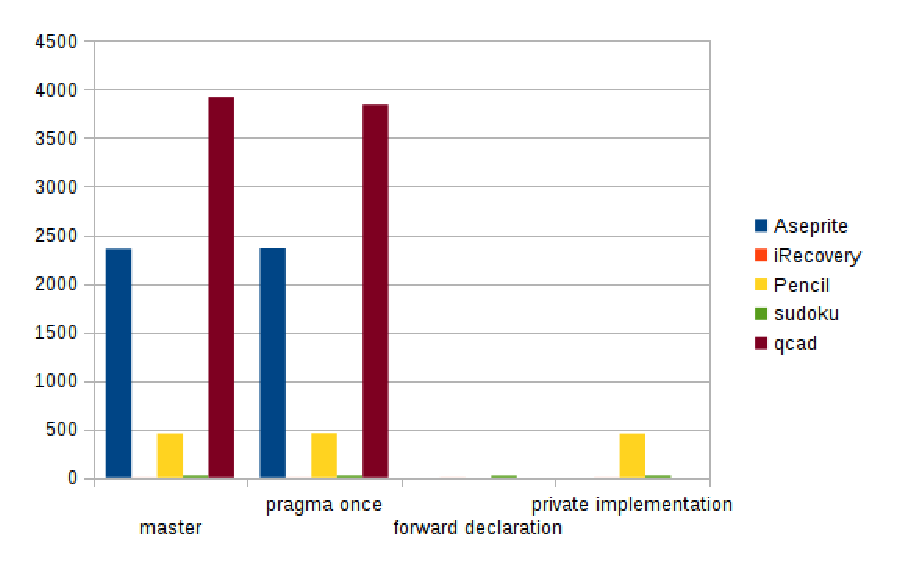
\includegraphics{figuras/graficos/linux_alteracao_codigo.eps}
    \caption{Dados Coletados - Alteração de Código no Linux}
    \label{benchmark_guardas_de_inclusao}
\end{figure}

\begin{figure}[b]
    \centering
        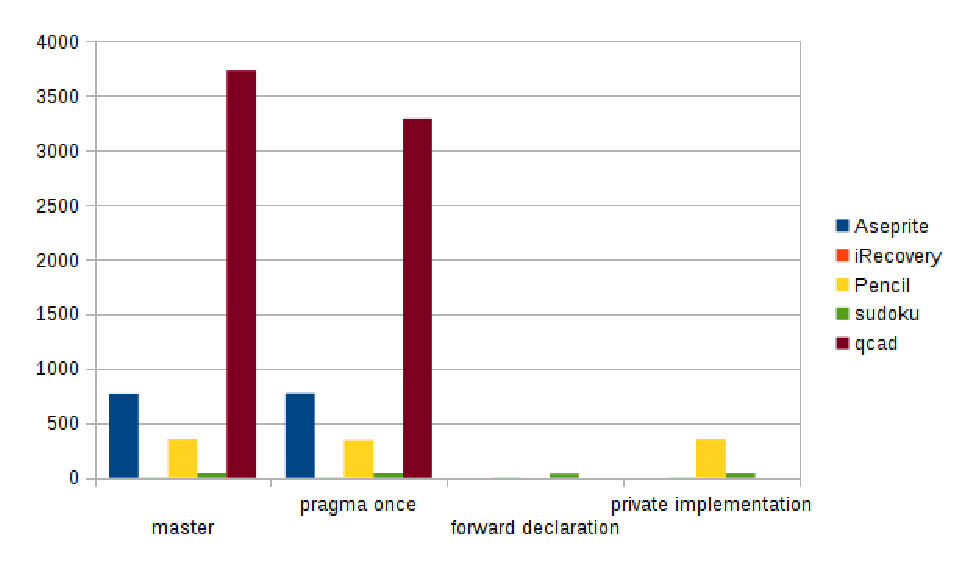
\includegraphics{figuras/graficos/mac_os_alteracao_codigo.eps}
    \caption{Dados Coletados - Alteração de Código no Mac OS Yosemite}
    \label{benchmark_guardas_de_inclusao}
\end{figure}

\begin{figure}[b]
    \centering
        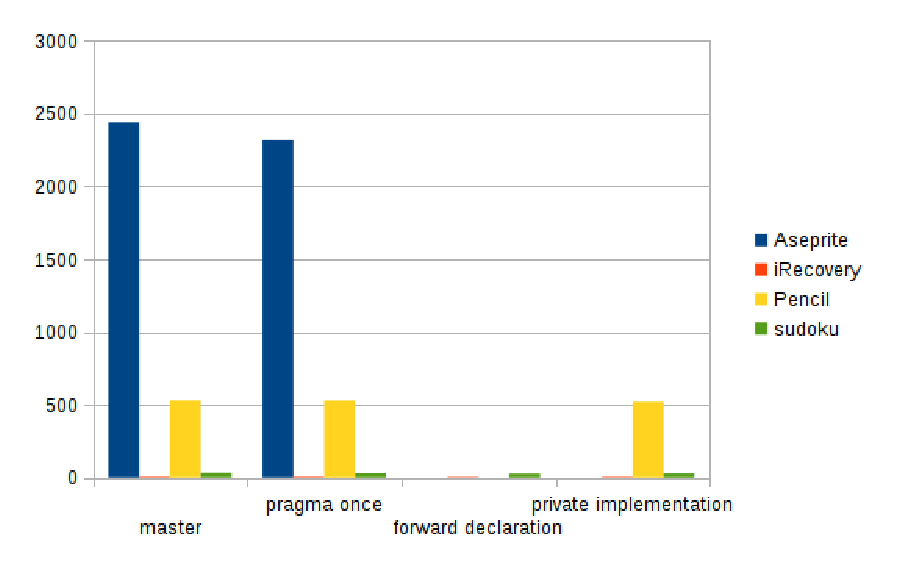
\includegraphics{figuras/graficos/windows_alteracao_codigo.eps}
    \caption{Dados Coletados - Alteração de Código no Windows 7}
    \label{benchmark_guardas_de_inclusao}
\end{figure}


\begin{itemize}
    \item Analise
    \subitem Depois da coleta de dados e fazendo simples calculos conclui-se que:

    \begin{enumerate}
       \item Em projetos a utilização do \texttt{\#pragma once} não possui interferência
 significativa no tempo de compilação dos projetos, uma vez que no maior
 projeto(QCAD) o tempo de compilação foi reduzido em 11.77\% e a remoção
 do \texttt{\#pragma once} no projeto aseprite resultou em uma redução de 5\%;
        \item Como a aplicação do método \textit{forward declaration} foi feita em projetos 
com tempo de compilação baixo, a diferença foi pouco perceptivel,
 com um valor máximo de 5\% na redução, no entanto ocorreu uma redução em todos os casos;
        \item A aplicação do método \textit{pimpl} não possui uma interferência direta
 no tempo de compilação, uma vez que este método possui efeito na modularização
 e promover a interdependência entre os headers, o que melhora a recompilação de
 um projeto, caso os objetos intermediários da compilação não sejam removidos.
    \end{enumerate}
\end{itemize}

\clearpage
\subsection{Alteração de flags de Otimização}

\begin{itemize}
    \item Tabelas e Gráficos
\end{itemize}

\subsubsection*{Aseprite}

%PROJETO ASEPRITE TABELAS 
\begin{table}[!ht]
\tiny
\centering
\caption{Aseprite - Flags de Otimização da Compilação no Linux}
\label{tab:otimizacao_compilacao:linux:aseprite}
\begin{tabular}{llllllll}
\textbf{Aseprite} & \textbf{-O}  & \textbf{-O0}   & \textbf{-O2} & \textbf{-O3} & \textbf{-Os} & \textbf{-Ofast} & \textbf{-Og} \\ \toprule
1                 & 2428.4120    & 2260.5384      & 2514.9207    & 2561.8271    & 2319.3125    &    842.4427     & 2385.7684  \\ 
2                 & 2271.3874    & 2051.0073      & 2333.7905    & 2384.6942    & 2235.8169    &    694.0581     & 2243.8749  \\ 
3                 & 2241.6417    & 2050.1224      & 2352.6054    & 2374.5866    & 2236.5715    &    694.0660     & 2238.7497  \\ 
4                 & 2269.4441    & 2053.0067      & 2341.8494    & 2419.4744    & 2235.4428    &    688.8936     & 2232.4368  \\ 
5                 & 2270.0459    & 2054.9605      & 2326.8056    & 2397.2705    & 2236.9505    &    691.6836     & 2244.6255  \\ 
6                 & 2244.0567    & 2059.6010      & 2342.5205    & 2387.0151    & 2239.6219    &    686.9482     & 2250.8028  \\ 
7                 & 2249.4974    & 2053.8001      & 2339.0471    & 2402.3641    & 2250.0025    &    689.9473     & 2228.1283  \\ 
8                 & 2266.6575    & 2043.2351      & 2335.0176    & 2413.0873    & 2234.3189    &    690.0143     & 2230.7049  \\ 
9                 & 2240.5459    & 2055.2829      & 2344.1943    & 2372.7927    & 2232.4647    &    689.7057     & 2233.7111  \\ 
10                & 2263.4064    & 2051.9990      & 2347.9277    & 2410.9841    & 2246.9743    &    688.1589     & 2247.4484  \\ \bottomrule
Média             & 2274.5095    & 2073.3554      & 2357.8679    & 2412.4096    & 2246.7476    &    705.5919     & 2253.6251  \\ 
\end{tabular}
\end{table}

\begin{table}[!ht]
\tiny
\centering
\caption{Aseprite - Flags de Otimização da Compilação no Mac OS Yosemite}
\label{tab:otimizacao_compilacao:mac:aseprite}
\begin{tabular}{llllllll}
\textbf{Aseprite} & \textbf{-O}  & \textbf{-O0}   & \textbf{-O2} & \textbf{-O3} & \textbf{-Os} & \textbf{-Ofast} & \textbf{-Og} \\ \toprule
1                 & 788.1713     &  609.0200      &  788.2866    & 806.1006     &  730.4503  &   224.4995        &  -           \\ 
2                 & 769.4564     &  590.3682      &  767.4185    & 798.2425     &  710.3456  &   207.2422        &  -           \\ 
3                 & 774.6238     &  590.3272      &  764.6951    & 789.8889     &  703.9241  &   207.2004        &  -           \\ 
4                 & 773.4311     &  589.9075      &  764.9236    & 795.9168     &  713.1742  &   208.3290        &  -           \\ 
5                 & 774.2611     &  593.2329      &  779.1553    & 793.6047     &  711.7219  &   207.1859        &  -           \\ 
6                 & 776.9802     &  591.1526      &  763.0460    & 798.4333     &  710.8471  &   208.0186        &  -           \\ 
7                 & 772.8281     &  592.0193      &  764.7422    & 789.6653     &  697.3718  &   206.0125        &  -           \\ 
8                 & 774.9873     &  589.5759      &  768.9518    & 793.2364     &  697.7304  &   207.3992        &  -           \\ 
9                 & 776.6190     &  587.6340      &  764.8288    & 794.2100     &  703.1416  &   208.1880        &  -           \\ 
10                & 775.5665     &  589.8825      &  765.5380    & 794.8966     &  703.5831  &   207.0215        &  -           \\ \bottomrule
Média             & 775.6925     &  592.3120      &  769.1586    & 795.4195     &  708.2290  &   209.1097        &  -           \\ 
\end{tabular}
\end{table}

\begin{table}[!ht]
\tiny
\centering
\caption{aseprite - flags de otimização da compilação no Windows 7}
\label{tab:otimizacao_compilacao:windows:aseprite}
\begin{tabular}{llllllll}
\textbf{Aseprite} & \textbf{-O}  & \textbf{-O0}   & \textbf{-O2} & \textbf{-O3} & \textbf{-Os} & \textbf{-Ofast} & \textbf{-Og} \\ \toprule
1                 &  2285.9375   &  2141.9688     & 2504.0313    &  2606.3594   &  2248.0625   & 665.9063        &  2219.0781   \\ 
2                 &  2240.8438   &  2088.2188     & 2462.2656    &  2561.1094   &  2226.4375   & 611.2656        &  2172.0469   \\ 
3                 &  2238.7656   &  2094.9844     & 2429.9063    &  2544.8281   &  2217.8281   & 618.2188        &  2198.7031   \\ 
4                 &  2241.7813   &  2083.4375     & 2419.6250    &  2570.2813   &  2197.9531   & 618.3594        &  2173.2188   \\ 
5                 &  2264.3906   &  2079.0625     & 2436.5938    &  2539.1250   &  2223.7500   & 618.6875        &  2190.4688   \\ 
6                 &  2265.3438   &  2072.4063     & 2413.1406    &  2565.3438   &  2194.9219   & 620.8125        &  2205.1406   \\ 
7                 &  2285.8125   &  2093.2969     & 2444.6719    &  2549.6704   &  2248.1875   & 605.1094        &  2183.9844   \\ 
8                 &  2220.1406   &  2104.7813     & 2437.4375    &  2503.6875   &  2271.7500   & 613.6875        &  2160.1563   \\ 
9                 &  2225.7813   &  2084.2188     & 2437.3125    &  2525.3281   &  2260.6563   & 618.3750        &  2168.8750   \\ 
10                &  2273.6563   &  2081.7500     & 2428.8438    &  2540.9219   &  2222.4375   & 617.4063        &  2174.0313   \\ \bottomrule
média             &  2254.2453   &  2092.4125     & 2441.3828    &  2550.6655   &  2231.1984   & 620.7828        &  2184.5703   \\ 
\end{tabular}
\end{table}

\clearpage
\subsubsection*{iRecoveryplusplus}
%PROJETO IRECOVERYPLUSPLUS TABELAS 

\begin{table}[!ht]
\tiny
\centering
\caption{iRecoveryplusplus - Flags de Otimização da Compilação no Linux}
\label{tab:otimizacao_compilacao:linux:irecoveryplusplus}
\begin{tabular}{llllllll}
\textbf{iRecoveryplusplus} & \textbf{-O}  & \textbf{-O0}   & \textbf{-O2} & \textbf{-O3} & \textbf{-Os} & \textbf{-Ofast} & \textbf{-Og} \\ \toprule
1                          & 1.0295       &   0.9205       &  1.1434      &   1.1348     & 0.9329       &   1.1792        &  1.0145      \\ 
2                          & 1.0814       &   0.9904       &  1.0827      &   1.0842     & 0.9084       &   1.1016        &  1.0078      \\ 
3                          & 0.9600       &   0.8296       &  1.1257      &   1.0619     & 0.8918       &   1.1663        &  0.9889      \\ 
4                          & 1.0160       &   0.8750       &  1.0751      &   1.2117     & 0.9385       &   1.1320        &  1.1048      \\ 
5                          & 1.0283       &   0.8781       &  1.0623      &   1.1440     & 0.8397       &   1.1591        &  0.9839      \\ 
6                          & 0.9734       &   0.8727       &  1.1633      &   1.1056     & 0.8799       &   1.1107        &  1.0287      \\ 
7                          & 1.0707       &   0.9437       &  1.0963      &   1.0816     & 0.9179       &   1.1152        &  0.9979      \\ 
8                          & 1.0478       &   0.9299       &  1.4273      &   1.1642     & 0.8657       &   1.1052        &  1.0088      \\ 
9                          & 1.0554       &   0.8168       &  1.0871      &   1.1080     & 0.8483       &   1.0804        &  1.0800      \\ 
10                         & 1.1668       &   0.8495       &  1.4181      &   1.0897     & 0.9279       &   1.1124        &  1.0608      \\ \bottomrule
Média                      & 1.0429       &   0.8906       &  1.1681      &   1.1186     & 0.8951       &   1.1262        &  1.0276      \\ 
\end{tabular}
\end{table}

\begin{table}[!ht]
\tiny
\centering
\caption{iRecoveryplusplus - Flags de Otimização da Compilação no Mac OS Yosemite}
\label{tab:otimizacao_compilacao:mac:irecoveryplusplus}
\begin{tabular}{llllllll}
\textbf{iRecoveryplusplus} & \textbf{-O}  & \textbf{-O0}   & \textbf{-O2} & \textbf{-O3} & \textbf{-Os} & \textbf{-Ofast} & \textbf{-Og} \\ \toprule
1                          & 3.3391       &   2.7805       &  2.7747      &  2.8193      &  2.8152      &   2.8780        &  -           \\ 
2                          & 2.8881       &   2.8706       &  2.9096      &  2.8318      &  3.1142      &   2.8373        &  -           \\ 
3                          & 2.8863       &   2.7529       &  2.8155      &  2.8035      &  2.6651      &   2.8276        &  -           \\ 
4                          & 2.7618       &   2.2722       &  2.8629      &  2.9031      &  2.6988      &   2.8334        &  -           \\ 
5                          & 2.9073       &   2.3670      &  2.8847      &  2.8012      &  3.1920      &   2.8224        &  -           \\ 
6                          & 2.8206       &   2.9688      &  2.8877      &  2.8034      &  2.7669      &   2.8981        &  -           \\ 
7                          & 2.8961       &   2.7507      &  2.8877      &  2.8764      &  2.5998      &   2.8582        &  -           \\ 
8                          & 2.8205       &   2.7768      &  2.8634      &  2.8438      &  2.6642      &   2.8989        &  -           \\ 
9                          & 2.8858       &   2.1318      &  2.7734      &  2.7415      &  2.6096      &   2.8480        &  -           \\ 
10                         & 2.7613       &   2.0424      &  2.8015      &  2.9054      &  2.5198      &   2.9179        &  -           \\ \bottomrule
Média                      & 2.8967       &   2.5714      &  2.8461      &  2.8329      &  2.7646      &   2.8620        &  -           \\ 
\end{tabular}
\end{table}


\begin{table}[!ht]
\tiny
\centering
\caption{iRecoveryplusplus - flags de otimização da compilação no Windows 7}
\label{tab:otimizacao_compilacao:windows:irecoveryplusplus}
\begin{tabular}{llllllll}
\textbf{iRecoveryplusplus} & \textbf{-O}  & \textbf{-O0}   & \textbf{-O2} & \textbf{-O3} & \textbf{-Os} & \textbf{-Ofast} & \textbf{-Og} \\ \toprule
1                          &   4.2969     &    5.2656      & 4.4375       & 4.9219       &  4.8438      &   4.7656        &  5.2813  \\ 
2                          &   4.4219     &    4.7031      & 4.7969       & 5.0625       &  4.8125      &   5.2188        &  4.9844  \\ 
3                          &   4.7500     &    4.8125      & 4.7969       & 5.3594       &  4.4375      &   4.4688        &  4.6406  \\ 
4                          &   4.6094     &    4.5625      & 4.8438       & 4.9375       &  4.3750      &   5.2031        &  4.3906  \\ 
5                          &   4.6094     &    4.6094      & 5.1094       & 4.9531       &  4.3438      &   5.3594        &  4.7031  \\ 
6                          &   4.4375     &    4.3438      & 5.6875       & 5.6406       &  4.5000      &   5.6406        &  4.8438  \\ 
7                          &   4.3750     &    4.8281      & 5.0625       & 5.1563       &  4.5156      &   4.7969        &  4.4688  \\ 
8                          &   4.5781     &    4.8750      & 5.1719       & 4.9531       &  4.3281      &   4.7656        &  5.2656  \\ 
9                          &   4.6719     &    4.5156      & 5.0156       & 5.4063       &  4.3750      &   4.7031        &  4.8125  \\ 
10                         &   5.0625     &    3.9688      & 4.7656       & 5.2656       &  4.7500      &   4.5313        &  5.1563  \\ \bottomrule
média                      &   4.5813     &    4.6484      & 4.9688       & 5.1656       &  4.5281      &   4.9453        &  4.8547  \\ 
\end{tabular}
\end{table}

\clearpage
\subsubsection*{Pencil}
%PROJETO PENCIL TABELAS 

\begin{table}[!ht]
\tiny
\centering
\caption{Pencil - Flags de Otimização da Compilação no Linux}
\label{tab:otimizacao_compilacao:linux:pencil}
\begin{tabular}{llllllll}
\textbf{Pencil}            & \textbf{-O}  & \textbf{-O0}   & \textbf{-O2} & \textbf{-O3} & \textbf{-Os} & \textbf{-Ofast} & \textbf{-Og} \\ \toprule
1                          & 455.4740     &   453.7972     &  455.6515    &   454.3954   &   461.3637   &   454.6087      &   461.1411       \\ 
2                          & 458.5687     &   453.0420     &  458.6480    &   455.8612   &   451.2379   &   456.3201      &   457.7603       \\ 
3                          & 456.1341     &   453.2612     &  453.9845    &   456.0386   &   451.0199   &   452.0644      &   452.1741       \\ 
4                          & 455.9241     &   453.6109     &  452.3321    &   455.1617   &   451.8650   &   458.3650      &   454.3638       \\ 
5                          & 455.0626     &   456.3227     &  456.3933    &   452.7784   &   451.1833   &   456.5019      &   453.1567       \\ 
6                          & 454.6253     &   456.1635     &  452.3841    &   458.7813   &   452.3104   &   458.1658      &   451.5917       \\ 
7                          & 456.1520     &   461.9098     &  455.8518    &   452.1305   &   453.0904   &   452.4355      &   455.8444       \\ 
8                          & 456.0375     &   451.5324     &  454.1806    &   456.6440   &   456.5508   &   455.4595      &   454.2039       \\ 
9                          & 457.7828     &   453.7152     &  455.4113    &   453.6454   &   451.1968   &   452.4086      &   455.3102       \\ 
10                         & 459.6924     &   453.2093     &  455.8023    &   455.0911   &   452.3534   &   450.9296      &   451.3153       \\ \bottomrule
Média                      & 456.5454     &   454.6564     &  455.0640    &   455.0528   &   453.2172   &   454.7259      &   454.6861       \\ 
\end{tabular}
\end{table}


\begin{table}[!ht]
\centering
\tiny
\caption{Pencil - Flags de Otimização da Compilação no Mac OS Yosemite}
\label{tab:otimizacao_compilacao:mac:pencil}
\begin{tabular}{llllllll}
\textbf{Pencil}         & \textbf{-O}  & \textbf{-O0}   & \textbf{-O2} & \textbf{-O3} & \textbf{-Os} & \textbf{-Ofast} & \textbf{-Og} \\ \toprule
1                       & 355.3439     &   353.7290     &    355.0881  &    352.6608  &   349.1689   &   352.7384      &  -           \\ 
2                       & 353.1613     &   356.1727     &    352.3484  &    355.5543  &   369.1497   &   358.3245      &  -           \\ 
3                       & 352.5484     &   351.8661     &    353.0415  &    352.5796  &   375.6915   &   353.3902      &  -           \\ 
4                       & 352.7343     &   352.1315     &    352.9057  &    354.8242  &   376.2380   &   353.5124      &  -           \\ 
5                       & 353.0833     &   352.2203     &    352.1713  &    352.5561  &   378.8831   &   352.5611      &  -           \\ 
6                       & 352.6301     &   353.4998     &    352.2540  &    353.6754  &   378.1887   &   352.6806      &  -           \\ 
7                       & 353.3471     &   352.6812     &    352.2950  &    352.3423  &   357.7742   &   352.1714      &  -           \\ 
8                       & 353.5499     &   351.6440     &    352.9621  &    354.2137  &   354.8617   &   353.5657      &  -           \\ 
9                       & 352.6414     &   352.4142     &    353.0637  &    352.8731  &   356.9490   &   381.1381      &  -           \\ 
10                      & 352.0240     &   352.5088     &    354.2621  &    352.7468  &   351.7314   &   353.2352      &  -           \\ \bottomrule
Média                   & 353.1064     &   352.8868     &    353.0392  &    353.4026  &   364.8636   &   356.3318      &  -           \\ 
\end{tabular}
\end{table}

\begin{table}[!ht]
\centering
\tiny
\caption{Pencil - flags de otimização da compilação no Windows 7}
\label{tab:otimizacao_compilacao:windows:pencil}
\begin{tabular}{llllllll}
\textbf{Pencil}    & \textbf{-O}  & \textbf{-O0}   & \textbf{-O2} & \textbf{-O3} & \textbf{-Os} & \textbf{-Ofast} & \textbf{-Og} \\ \toprule
1                  & 520.0625     &   500.8906     &    538.3750  &    538.0469  &    543.6563  &   543.0938      &   506.2969       \\ 
2                  & 523.6406     &   508.5938     &    521.5781  &    529.4375  &    524.0000  &   532.3906      &   505.2188       \\ 
3                  & 514.5313     &   494.6250     &    532.3281  &    533.5000  &    526.1094  &   534.9531      &   514.7344       \\ 
4                  & 531.6563     &   503.0781     &    528.8750  &    534.0938  &    512.1563  &   549.3750      &   512.7656       \\ 
5                  & 517.6875     &   505.2656     &    533.0938  &    533.9844  &    522.9063  &   547.5000      &   505.3750       \\ 
6                  & 511.5781     &   501.7969     &    530.6719  &    529.0625  &    509.9063  &   527.2344      &   516.5313       \\ 
7                  & 510.3594     &   498.9375     &    531.1250  &    532.8594  &    529.4063  &   537.8750      &   520.0781       \\ 
8                  & 509.7500     &   503.4375     &    538.9375  &    538.9063  &    517.6094  &   542.6250      &   520.8750       \\ 
9                  & 516.4531     &   501.4063     &    528.5156  &    534.2813  &    522.5000  &   549.1719      &   513.1875       \\ 
10                 & 511.1563     &   500.8125     &    524.0313  &    541.3906  &    520.8438  &   534.9688      &   524.3125       \\ \bottomrule
média              & 516.6875     &   501.8844     &    530.7531  &    534.5563  &    522.9094  &   539.9188      &   513.9375       \\ 
\end{tabular}
\end{table}


\clearpage
\subsubsection*{Sudoku}
%PROJETO SUDOKU TABELAS 

\begin{table}[!ht]
\centering
\tiny
\caption{Sudoku - Flags de Otimização da Compilação no Linux}
\label{tab:otimizacao_compilacao:linux:sudoku}
\begin{tabular}{llllllll}
\textbf{Sudoku}            & \textbf{-O}  & \textbf{-O0}   & \textbf{-O2} & \textbf{-O3} & \textbf{-Os} & \textbf{-Ofast} & \textbf{-Og} \\ \toprule
1                          & 23.5794      & 22.0289        & 22.1422      & 21.9497      & 19.6868      & 21.4870         & 21.9286    \\ 
2                          & 22.0800      & 22.4456        & 22.0332      & 21.9361      & 19.5858      & 22.0021         & 22.0167    \\ 
3                          & 22.0984      & 22.0593        & 21.7976      & 21.8664      & 19.8344      & 22.0210         & 21.7269    \\ 
4                          & 21.7172      & 22.1378        & 22.0241      & 21.6025      & 19.6490      & 21.9593         & 21.6730    \\ 
5                          & 22.3950      & 22.1298        & 25.4559      & 21.9436      & 19.4276      & 21.9457         & 22.3169    \\ 
6                          & 22.1307      & 22.1869        & 21.8995      & 21.9011      & 19.4698      & 22.0589         & 22.0904    \\ 
7                          & 22.0020      & 22.1432        & 21.9687      & 22.0499      & 19.5573      & 22.2119         & 23.1416    \\ 
8                          & 22.1447      & 22.2793        & 21.4932      & 22.0821      & 19.5723      & 21.7472         & 22.0980    \\ 
9                          & 22.0802      & 22.0366        & 21.5503      & 21.8815      & 20.0108      & 21.7302         & 21.9612    \\ 
10                         & 22.0947      & 25.6994        & 21.7469      & 21.9718      & 19.7197      & 22.0414         & 21.8521    \\ \bottomrule
Média                      & 22.2322      & 22.5147        & 22.2112      & 21.9185      & 19.6514      & 21.9205         & 22.0805    \\ 
\end{tabular}
\end{table}

\begin{table}[!ht]
\centering
\tiny
\caption{Sudoku - Flags de Otimização da Compilação no Mac OS Yosemite}
\label{tab:otimizacao_compilacao:mac:sudoku}
\begin{tabular}{llllllll}
\textbf{Sudoku}         & \textbf{-O}  & \textbf{-O0}   & \textbf{-O2} & \textbf{-O3} & \textbf{-Os} & \textbf{-Ofast} & \textbf{-Og} \\ \toprule
1                       & 38.3382      & 38.8962        & 38.2454      & 38.7424      & 39.4471      & 38.4162         &  -           \\ 
2                       & 38.5911      & 38.6555        & 38.3764      & 38.2607      & 39.3203      & 38.7771         &  -           \\ 
3                       & 38.6160      & 38.9842        & 38.6331      & 38.4287      & 39.3242      & 38.0117         &  -           \\ 
4                       & 37.9895      & 38.0715        & 38.4525      & 38.0314      & 39.4237      & 38.3163         &  -           \\ 
5                       & 38.4379      & 37.9539        & 38.6316      & 38.5387      & 39.2862      & 38.7696         &  -           \\ 
6                       & 38.1603      & 38.6485        & 38.2802      & 37.8681      & 39.3197      & 38.0426         &  -           \\ 
7                       & 38.4832      & 38.0982        & 38.0891      & 38.5532      & 39.4502      & 38.4225         &  -           \\ 
8                       & 38.3560      & 38.5092        & 38.0895      & 38.0421      & 39.4214      & 37.9470         &  -           \\ 
9                       & 38.2962      & 38.8282        & 38.7379      & 38.2293      & 39.3191      & 38.2541         &  -           \\ 
10                      & 38.3496      & 38.3687        & 38.6165      & 38.5052      & 39.4786      & 38.4714         &  -           \\ \bottomrule
Média                   & 38.3618      & 38.5014        & 38.4152      & 38.3200      & 39.3790      & 38.3428         &  -           \\ 
\end{tabular}
\end{table}

\begin{table}[!ht]
\centering
\tiny
\caption{Sudoku - flags de otimização da compilação no Windows 7}
\label{tab:otimizacao_compilacao:windows:sudoku}
\begin{tabular}{llllllll}
\textbf{Sudoku}    & \textbf{-O}  & \textbf{-O0}   & \textbf{-O2} & \textbf{-O3} & \textbf{-Os} & \textbf{-Ofast} & \textbf{-Og} \\ \toprule
1                  & 32.0469      & 29.0938        & 33.1406      & 35.9688      & 31.3281      & 35.5625         & 31.1563     \\ 
2                  & 31.8750      & 28.7500        & 31.2969      & 35.0156      & 30.3281      & 35.2813         & 29.8281     \\ 
3                  & 31.6719      & 29.9844        & 33.1406      & 35.0781      & 31.4844      & 34.5156         & 30.1094     \\ 
4                  & 30.7344      & 29.3594        & 32.0938      & 35.6094      & 31.8906      & 37.1563         & 29.9688     \\ 
5                  & 30.5000      & 30.2031        & 32.7500      & 36.0938      & 32.4688      & 36.4844         & 30.5156     \\ 
6                  & 30.7656      & 28.7188        & 32.3906      & 34.5156      & 32.2813      & 34.7813         & 29.1563     \\ 
7                  & 32.3750      & 28.4844        & 33.4063      & 34.2969      & 31.7656      & 35.3594         & 30.1563     \\ 
8                  & 29.4375      & 31.1094        & 33.5938      & 34.2500      & 30.0156      & 35.6406         & 30.3906     \\ 
9                  & 31.1563      & 27.4375        & 33.2969      & 37.2188      & 31.0781      & 36.6563         & 30.1719     \\ 
10                 & 30.9688      & 29.6406        & 32.1250      & 34.7188      & 31.4844      & 35.4688         & 29.6406     \\ \bottomrule
média              & 31.1531      & 29.2781        & 32.7234      & 35.2766      & 31.4125      & 35.6906         & 30.1094     \\ 
\end{tabular}
\end{table}

\clearpage
\subsubsection*{Qcad}
%PROJETO QCAD TABELAS 

\begin{table}[!ht]
\centering
\tiny
\caption{Qcad - Flags de Otimização da Compilação no Linux}
\label{tab:otimizacao_compilacao:linux:qcad}
\begin{tabular}{llllllll}
\textbf{Qcad}            & \textbf{-O}  & \textbf{-O0}   & \textbf{-O2} & \textbf{-O3} & \textbf{-Os} & \textbf{-Ofast} & \textbf{-Og} \\ \toprule
1                        & 3910.5869    &  3927.3261     &  3922.6279   &   3918.3749  &   3890.4638  &    3921.3795    &   3951.2642           \\ 
2                        & 3920.6295    &  3925.3639     &  3924.2405   &   3916.5140  &   3884.8599  &    3921.8527    &   4004.5549           \\ 
3                        & 3918.1448    &  3922.5499     &  3918.2415   &   3911.9738  &   3881.8755  &    3929.4902    &   3926.3707           \\ 
4                        & 3919.6268    &  3925.5230     &  3927.2388   &   3915.1442  &   3887.1729  &    3915.2546    &   3929.2216           \\ 
5                        & 3913.3476    &  3923.8203     &  3909.7712   &   3922.1575  &   3885.4041  &    3924.2709    &   3924.1439           \\ 
6                        & 3922.7388    &  3927.4205     &  3922.4313   &   3918.6355  &   3888.2514  &    3926.2758    &   3928.1144           \\ 
7                        & 3915.4064    &  3925.0573     &  3915.6719   &   3926.8127  &   3885.4175  &    3925.8235    &   3934.5177           \\ 
8                        & 3938.8978    &  3926.8358     &  3934.1575   &   3913.8567  &   3888.2649  &    3923.7448    &   3922.4567           \\ 
9                        & 3917.2526    &  3922.5346     &  3929.0349   &   3935.2480  &   3887.3314  &    3913.7215    &   3928.7853           \\ 
10                       & 3915.1611    &  3930.4288     &  3927.5069   &   3919.6895  &   3886.5140  &    3927.3606    &   3924.2721           \\ \bottomrule
Média                    & 3919.1792    &  3925.6860     &  3923.0922   &   3919.8407  &   3886.5556  &    3922.9174    &   3937.3701           \\ 
\end{tabular}
\end{table}

\begin{table}[!ht]
\centering
\tiny
\caption{Qcad - Flags de Otimização da Compilação no Mac OS Yosemite}
\label{tab:otimizacao_compilacao:mac:qcad}
\begin{tabular}{llllllll}
\textbf{Qcad}         & \textbf{-O}  & \textbf{-O0}   & \textbf{-O2} & \textbf{-O3} & \textbf{-Os} & \textbf{-Ofast} & \textbf{-Og} \\ \toprule
1                     & 3851.4074    &   3109.9399    &   3738.2187  &   3748.0183  &   3796.1528  &   3802.1043     &  -           \\ 
2                     & 3791.8801    &   3078.3796    &   3748.0250  &   3735.7577  &   3784.8870  &   3786.2843     &  -           \\ 
3                     & 3798.0112    &   3082.0572    &   3727.1546  &   3737.6603  &   3775.5470  &   3780.0927     &  -           \\ 
4                     & 3788.9006    &   3068.2094    &   3722.7333  &   3735.4360  &   3820.6566  &   3779.5674     &  -           \\ 
5                     & 3793.7368    &   3076.9819    &   3722.3808  &   3735.6313  &   3782.0788  &   3778.3790     &  -           \\ 
6                     & 3790.2542    &   3076.4253    &   3727.3305  &   3738.1959  &   3793.0921  &   3782.9355     &  -           \\ 
7                     & 3789.6725    &   3079.1327    &   3729.9403  &   3738.1217  &   3790.3613  &   3808.3038     &  -           \\ 
8                     & 3782.4943    &   3073.7092    &   3722.0891  &   3738.1959  &   3786.5515  &   3789.3795     &  -           \\ 
9                     & 3789.4735    &   3072.3970    &   3731.7932  &   3735.1269  &   3835.3118  &   3776.1316     &  -           \\ 
10                    & 3783.6960    &   3074.5065    &   3728.2715  &   3736.6376  &   3772.8905  &   3782.6756     &  -           \\ \bottomrule
Média                 & 3795.9526    &   3079.1739    &   3729.7937  &   3737.8782  &   3793.7529  &   3786.5854     &  -           \\ 
\end{tabular}
\end{table}


        
\begin{figure}[!h]
    \centering
        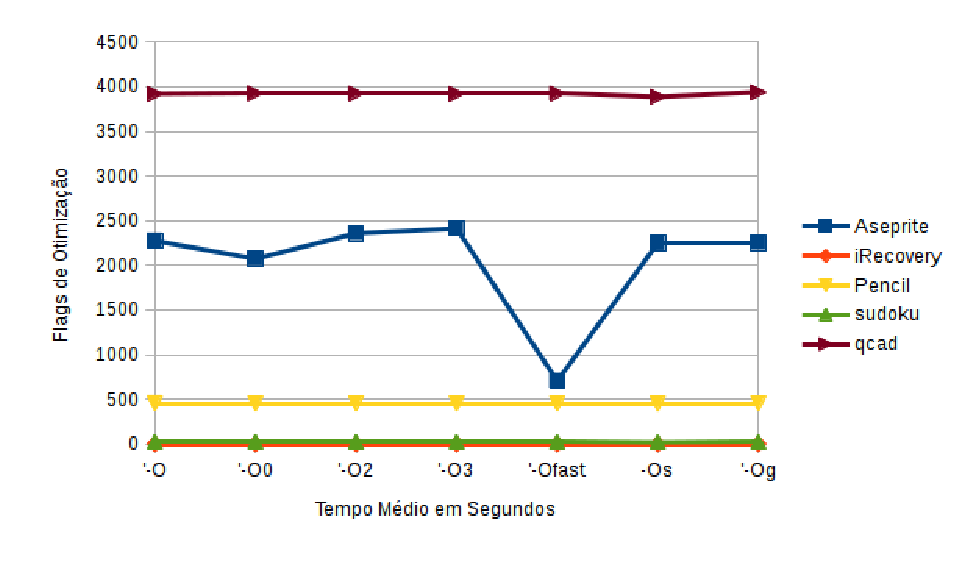
\includegraphics{figuras/graficos/linux_otimizacao.eps}
    \caption{Dados Coletados - Utilização de Flags de Otimização no Linux}
    \label{flags_de_otimizacao_linux}
\end{figure}

\begin{figure}[!h]
    \centering
        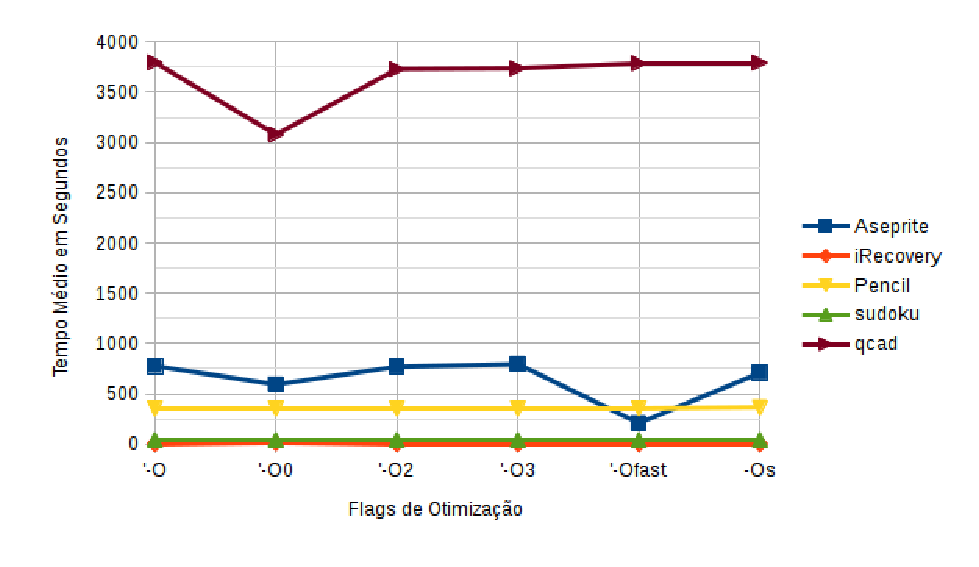
\includegraphics{figuras/graficos/mac_os_otimizacao.eps}
    \caption{Dados Coletados - Utilização de Flags de Otimização no Mac OS Yosemite}
    \label{flags_de_otimizacao_mac_os}
\end{figure}


\begin{figure}[!h]
    \centering
        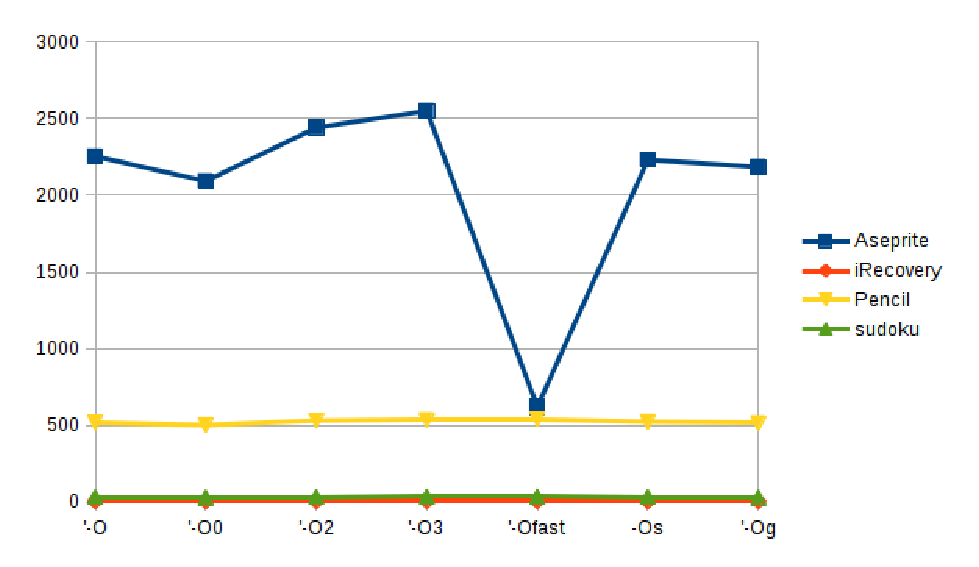
\includegraphics{figuras/graficos/windows_otimizacao.eps}
    \caption{Dados Coletados - Utilização de Flags de Otimização no Windows 7}
    \label{flags_de_otimizacao_windows}
\end{figure}

\begin{itemize}
    \item Analise

        Com a coleta de dados e a analise dos gráficos conclue-se:

        \begin{enumerate}
            \item Analisando os projetos que utilizão qmake como gerador de \textit{makefile}
 as flags de otimização não tiveram uma grande impacto no tempo de otmização, como mostrado nos gráficos 
o tempo foi linear. 
            \item Analisando o projeto que possui como gerador de \textit{makefile} como
 \textit{cmake} a \textit{flag} \textbf{-Ofast} obteve o menor tempo de redução, com um impacto
 significativo de aproximadamente de 70\% a 75\% em todos os ambientes.
            \item  Analisando o maior projeto, o tempo de compilação foi reduzido utilizando-se a
 flag -O0, no entanto este fato ocorreu apenas em ambiente Mac OS Yosemite, no ambiente linux independente
 da flag de otimização o tempo de compilação variou linearmente com variação quase imperceptível.
        \end{enumerate}
\end{itemize}



\clearpage
\subsection{Alteração de flags de processamento paralelo}

\begin{itemize}
    \item Tabelas e Gráficos
\end{itemize}


\subsubsection*{Aseprite}
%PROJETO ASEPRITE TABELAS 

\begin{table}[!ht]
\centering
\tiny
\caption{Aseprite - Flags de Processamento Paralelo no Linux}
\label{tab:flag_processamento_paralelo:linux:aseprite}
\begin{tabular}{llllll}
\textbf{Aseprite} & \textbf{-j 2} & \textbf{-j 4} & \textbf{-j 6} & \textbf{-j 8} & \textbf{-j10}  \\ \toprule
1                 &  1422.5747    &     1220.9304 &     1251.0829 &     1762.8992 &  1516.1982    \\ 
2                 &  1373.0582    &     1245.3321 &     1269.7347 &     1805.3795 &  1635.7142    \\ 
3                 &  1392.4281    &     1211.2491 &     1416.2245 &     1742.7766 &  1502.8607    \\ 
4                 &  1383.2098    &     1240.3822 &     1426.8681 &     1780.4778 &  1473.9050    \\ 
5                 &  1421.0623    &     1246.5464 &     1402.7551 &     1688.7998 &  1368.8088    \\ 
6                 &  1375.9400    &     1217.6862 &     1566.9732 &     1691.2214 &  1487.2643    \\ 
7                 &  1385.9952    &     1228.6808 &     1550.1486 &     1602.3923 &  1358.4499    \\ 
8                 &  1383.6518    &     1235.4873 &     1545.7303 &     1606.4604 &  1382.3776    \\ 
9                 &  1391.0771    &     1218.4570 &     1661.1944 &     1625.7141 &  1332.0942    \\ 
10                &  1373.0357    &     1231.2301 &     1700.1015 &     1648.5087 &  1335.5501    \\ \bottomrule
Média             &  1390.2033    &     1229.5982 &     1479.0813 &     1695.4630 &  1439.3223    \\ 
\end{tabular}
\end{table}

\begin{table}[!ht]
\centering
\tiny
\caption{Aseprite - Flags de Processamento Paralelo no Mac OS Yosemite}
\label{tab:flag_processamento_paralelo:mac:aseprite}
\begin{tabular}{llllll}
\textbf{Aseprite} & \textbf{-j 2} & \textbf{-j 4} & \textbf{-j 6} & \textbf{-j 8} & \textbf{-j10}  \\ \toprule
1                 & 578.2032      &   575.9309    &    288.9686   &     580.5286  &   573.5415  \\ 
2                 & 577.5507      &   576.2220    &    284.9080   &     575.5498  &   572.1267  \\ 
3                 & 573.9103      &   574.6409    &    291.1655   &     577.6787  &   571.5593  \\ 
4                 & 580.5016      &   574.7476    &    283.9961   &     574.0696  &   570.0263  \\ 
5                 & 578.5848      &   584.5247    &    293.5214   &     581.9131  &   572.7821  \\ 
6                 & 569.2962      &   573.2728    &    287.2380   &     573.4792  &   570.0864  \\ 
7                 & 575.6596      &   577.6826    &    297.1421   &     577.1653  &   571.5139  \\ 
8                 & 576.9742      &   575.4852    &    284.0043   &     575.7631  &   575.3054  \\ 
9                 & 572.6335      &   572.9737    &    286.6796   &     587.5273  &   572.6971  \\ 
10                & 578.8830      &   573.0292    &    288.5725   &     581.3931  &   570.0729  \\ \bottomrule
Média             & 576.2197      &   575.8510    &    288.6196   &     578.5068  &   571.9712  \\ 
\end{tabular}
\end{table}


\begin{table}[!ht]
\centering
\tiny
\caption{Aseprite - Flags de Processamento Paralelo no Windows 7}
\label{tab:flag_processamento_paralelo:windows:aseprite}
\begin{tabular}{llllll}
\textbf{Aseprite} & \textbf{-j 2} & \textbf{-j 4} & \textbf{-j 6} & \textbf{-j 8} & \textbf{-j10}  \\ \toprule
1                 & 1049.8281     &   1675.8594   &   996.0781    &   1006.1094   &   982.7031     \\ 
2                 & 1068.8594     &   1024.8906   &   1008.6094   &   1033.1094   &   1006.5469    \\ 
3                 & 1068.0000     &   1053.7656   &   1012.0156   &   1057.8125   &   995.0156     \\ 
4                 & 1055.6719     &   1017.4844   &   1042.8125   &   1022.9531   &   1022.6563    \\ 
5                 & 1893.3594     &   1026.8438   &   984.4688    &   1654.8281   &   1081.9063    \\ 
6                 & 1051.6250     &   1025.9063   &   994.5938    &   991.8906    &   1005.9063    \\ 
7                 & 1043.4844     &   1006.3750   &   984.7969    &   1024.9375   &   1083.8125    \\ 
8                 & 1026.1563     &   1030.8906   &   1021.8281   &   1025.7188   &   1012.0313    \\ 
9                 & 1054.3906     &   1016.9063   &   995.9375    &   987.7344    &   1027.6719    \\ 
10                & 1093.0457     &   1052.2031   &   1014.5625   &   1027.0781   &   1003.6719    \\ \bottomrule
Média             & 1140.4421     &   1093.1125   &   1005.5703   &   1083.2172   &   1022.1922    \\ 
\end{tabular}
\end{table}

\clearpage
\subsubsection*{iRecoveryplusplus}
%PROJETO IRECOVERYPLUSPLUS TABELAS 

\begin{table}[!ht]
\centering
\tiny
\caption{iRecoveryplusplus - Flags de Processamento Paralelo no Linux}
\label{tab:flag_processamento_paralelo:linux:irecoveryplusplus}
\begin{tabular}{llllll}
\textbf{iRecoveryplusplus} & \textbf{-j 2} & \textbf{-j 4} & \textbf{-j 6} & \textbf{-j 8} & \textbf{-j10}  \\ \toprule
1                          & 1.0505        &  1.1042       &  1.1375       &  1.1768       &  1.2381        \\ 
2                          & 1.1425        &  1.0676       &  1.1250       &  1.1250       &  1.1480        \\ 
3                          & 1.0713        &  1.1384       &  1.1802       &  1.1138       &  1.1431        \\ 
4                          & 1.0573        &  1.1268       &  1.1377       &  1.1276       &  1.0915        \\ 
5                          & 1.0711        &  1.1138       &  1.0949       &  1.1724       &  1.0612        \\ 
6                          & 1.0971        &  1.1096       &  1.1476       &  1.1160       &  1.0889        \\ 
7                          & 1.1430        &  1.1175       &  1.0717       &  1.1664       &  1.0710        \\ 
8                          & 1.1658        &  1.1102       &  1.1188       &  1.0840       &  1.1109        \\ 
9                          & 1.1004        &  1.1873       &  1.1020       &  1.1301       &  1.0492        \\ 
10                         & 1.1769        &  1.1074       &  1.1401       &  1.1275       &  1.1678        \\ \bottomrule
Média                      & 1.1076        &  1.1183       &  1.1255       &  1.1340       &  1.1170        \\ 
\end{tabular}
\end{table}

\begin{table}[!ht]
\centering
\tiny
\caption{iRecoveryplusplus - Flags de Processamento Paralelo no Mac OS Yosemite}
\label{tab:flag_processamento_paralelo:mac:irecoveryplusplus}
\begin{tabular}{llllll}
\textbf{iRecoveryplusplus} & \textbf{-j 2} & \textbf{-j 4} & \textbf{-j 6} & \textbf{-j 8} & \textbf{-j10}  \\ \toprule
1                          & 2.5285        &  2.4667       &  2.4553       &  2.5164       &  2.3501    \\ 
2                          & 2.4183        &  2.4778       &  2.4793       &  2.8648       &  2.3752    \\ 
3                          & 2.4020        &  2.4761       &  2.4876       &  2.3739       &  2.3293    \\ 
4                          & 2.5213        &  2.4334       &  2.5144       &  2.2883       &  2.4144    \\ 
5                          & 2.6159        &  2.5339       &  2.4667       &  2.3679       &  2.3648    \\ 
6                          & 2.3998        &  2.6463       &  2.5849       &  2.3490       &  2.2704    \\ 
7                          & 2.4843        &  2.8607       &  2.5522       &  2.2977       &  2.3059    \\ 
8                          & 2.4747        &  3.3727       &  2.4091       &  2.3212       &  2.2715    \\ 
9                          & 2.5370        &  3.7488       &  2.4847       &  2.3738       &  2.3484    \\ 
10                         & 2.5734        &  2.2980       &  2.5224       &  2.3703       &  2.2323    \\ \bottomrule
Média                      & 2.4955        &  2.7314       &  2.4957       &  2.4123       &  2.3262    \\ 
\end{tabular}
\end{table}

\begin{table}[!ht]
\centering
\tiny
\caption{iRecoveryplusplus - Flags de Processamento Paralelo no Windows 7}
\label{tab:flag_processamento_paralelo:windows:irecoveryplusplus}
\begin{tabular}{llllll}
\textbf{iRecoveryplusplus} & \textbf{-j 2} & \textbf{-j 4} & \textbf{-j 6} & \textbf{-j 8} & \textbf{-j10}  \\ \toprule
1                          & 5.2500        &  5.4688       &  5.3438       & 5.0938        & 4.8438      \\ 
2                          & 5.0625        &  4.9688       &  5.0781       &  4.7969       &  4.7656     \\ 
3                          & 5.0625        &  4.7500       &  4.7969       &  4.7969       &  4.4688     \\ 
4                          & 5.6250        &  5.1094       &  5.5781       &  4.8125       &  5.0938     \\ 
5                          & 4.4531        &  4.7344       &  4.4844       &  4.8281       &  5.2969     \\ 
6                          & 4.8281        &  4.9688       &  5.3438       &  5.5625       &  5.0781     \\ 
7                          & 5.4844        &  5.4531       &  5.3438       &  5.5156       &  4.8594     \\ 
8                          & 4.7656        &  5.1875       &  5.2188       &  4.8125       &  4.6406     \\ 
9                          & 4.7188        &  5.0625       &  5.0781       &  5.1563       &  5.4531     \\ 
10                         & 4.6250        &  4.4844       &  4.8750       &  4.7344       &  4.9375     \\ \bottomrule
Média                      & 4.9875        &  5.0188       &  5.1141       &  5.0109       &  4.9438     \\ 
\end{tabular}
\end{table}

\clearpage
\subsubsection*{Pencil}
%PROJETO PENCIL TABELAS 

\begin{table}[!ht]
\centering
\tiny
\caption{Pencil - Flags de Processamento Paralelo no Linux}
\label{tab:flag_processamento_paralelo:linux:pencil}
\begin{tabular}{llllll}
\textbf{Pencil} & \textbf{-j 2} & \textbf{-j 4} & \textbf{-j 6} & \textbf{-j 8} & \textbf{-j10}  \\ \toprule
1                  & 266.6753  &   253.7153   &  268.9541 &    276.5708 &    279.3204       \\ 
2                  & 262.8651  &   243.0800   &  262.3380 &    272.8050 &    280.6357       \\ 
3                  & 266.6512  &   243.8087   &  258.3085 &    306.8622 &    282.3581       \\ 
4                  & 272.8472  &   238.6624   &  255.1279 &    278.2493 &    286.3986       \\ 
5                  & 270.0952  &   252.4405   &  261.6647 &    278.8923 &    293.7820       \\ 
6                  & 268.6468  &   238.3732   &  254.2527 &    304.3434 &    295.9109       \\ 
7                  & 278.2018  &   239.3942   &  251.8955 &    277.3592 &    288.5821       \\ 
8                  & 267.8349  &   235.9468   &  255.4461 &    296.6876 &    290.8762       \\ 
9                  & 276.3785  &   233.7197   &  251.9725 &    279.4619 &    293.7961       \\ 
10                 & 287.0007  &   243.0883   &  257.5330 &    278.6919 &    294.9429       \\ \bottomrule
Média              & 271.7197  &   242.2229   &  257.7493 &    284.9924 &    288.6603       \\ 
\end{tabular}
\end{table}

\begin{table}[!ht]
\centering
\tiny
\caption{Pencil - Flags de Processamento Paralelo no Mac OS Yosemite}
\label{tab:flag_processamento_paralelo:mac:pencil}
\begin{tabular}{llllll}
\textbf{Pencil} & \textbf{-j 2} & \textbf{-j 4} & \textbf{-j 6} & \textbf{-j 8} & \textbf{-j10}  \\ \toprule
1               & 277.2427  &   271.1315 &    272.7361  &   259.9174  &   258.2276          \\ 
2               & 274.8589  &   269.8826 &    286.2105  &   279.3511  &   262.6175          \\ 
3               & 278.6200  &   259.0627 &    279.0144  &   273.6935  &   254.1095          \\ 
4               & 282.2052  &   287.5182 &    295.9949  &   276.3455  &   268.0471          \\ 
5               & 284.8937  &   274.3423 &    274.8261  &   285.8305  &   269.4830          \\ 
6               & 261.9388  &   280.4124 &    280.1616  &   273.0806  &   266.0093          \\ 
7               & 286.7162  &   276.5590 &    282.9505  &   291.1252  &   263.5765          \\ 
8               & 274.9455  &   288.0063 &    292.4211  &   275.3359  &   273.8602          \\ 
9               & 295.1950  &   281.7498 &    276.0287  &   273.9958  &   270.0857          \\ 
10              & 276.5680  &   266.3367 &    280.9690  &   275.4276  &   269.8175          \\ \bottomrule
Média           & 279.3184  &   275.5002 &    282.1313  &   276.4103  &   265.5834          \\ 
\end{tabular}
\end{table}

\begin{table}[!ht]
\centering
\tiny
\caption{Pencil - Flags de Processamento Paralelo no Windows 7}
\label{tab:flag_processamento_paralelo:windows:pencil}
\begin{tabular}{llllll}
\textbf{Pencil} & \textbf{-j 2} & \textbf{-j 4} & \textbf{-j 6} & \textbf{-j 8} & \textbf{-j10}  \\ \toprule
1               & 261.0156  &   256.7500 &    259.6094   &  258.4375 &    283.8438           \\ 
2               & 260.1094  &   256.6719 &    258.0625   &  258.2656 &    260.8125           \\ 
3               & 261.8281  &   258.1719 &    262.5313   &  260.3594 &    259.9063           \\ 
4               & 260.5469  &   266.9219 &    258.9688   &  258.5000 &    261.6250           \\ 
5               & 262.8438  &   257.8750 &    258.7031   &  260.4063 &    259.4531           \\ 
6               & 261.5625  &   272.9531 &    258.0469   &  260.0938 &    269.4531           \\ 
7               & 261.3594  &   256.6250 &    257.8594   &  259.8906 &    269.3125           \\ 
8               & 260.4375  &   258.4531 &    258.3594   &  259.0938 &    273.7656           \\ 
9               & 273.2188  &   257.5000 &    258.1406   &  258.1250 &    265.7500           \\ 
10              & 260.5938  &   257.5313 &    258.6875   &  258.3594 &    260.7656           \\ \bottomrule
Média           & 262.3516  &   259.9453 &    258.8969   &  259.1531 &    266.4688           \\ 
\end{tabular}
\end{table}

\clearpage
\subsubsection*{Sudoku}
%PROJETO SUDOKU TABELAS 

\begin{table}[!ht]
\centering
\tiny
\caption{Sudoku - Flags de Processamento Paralelo no Linux}
\label{tab:flag_processamento_paralelo:linux:sudoku}
\begin{tabular}{llllll}
\textbf{Sudoku} & \textbf{-j 2} & \textbf{-j 4} & \textbf{-j 6} & \textbf{-j 8} & \textbf{-j10}  \\ \toprule
1               & 13.1612 & 13.2105 & 13.4355 & 13.5550 & 11.1120  \\ 
2               & 12.8530 & 13.1811 & 13.4956 & 13.4440 & 9.7460   \\ 
3               & 19.6240 & 13.4466 & 13.3907 & 13.5685 & 10.4685  \\ 
4               & 13.1826 & 13.1441 & 13.2488 & 13.4200 & 10.1563  \\ 
5               & 13.2789 & 13.0709 & 13.3169 & 16.7792 & 10.2000  \\ 
6               & 13.0488 & 13.0823 & 13.2919 & 13.3107 & 10.1864  \\ 
7               & 12.7417 & 13.2555 & 13.3103 & 13.3844 & 10.2037  \\ 
8               & 13.1751 & 13.2540 & 13.3199 & 13.4822 & 9.6099   \\ 
9               & 12.8913 & 13.1655 & 13.5218 & 17.4005 & 10.2552  \\ 
10              & 13.0475 & 13.4313 & 13.6425 & 13.3221 & 10.7716  \\ \bottomrule
Média           & 13.7004 & 13.2242 & 13.3974 & 14.1667 & 10.2710  \\ 
\end{tabular}
\end{table}

\begin{table}[!ht]
\centering
\tiny
\caption{Sudoku - Flags de Processamento Paralelo no Mac OS Yosemite}
\label{tab:flag_processamento_paralelo:mac:sudoku}
\begin{tabular}{llllll}
\textbf{Sudoku} & \textbf{-j 2} & \textbf{-j 4} & \textbf{-j 6} & \textbf{-j 8} & \textbf{-j10}  \\ \toprule
1               & 27.9679 & 29.7784 & 26.7719 & 29.8711 & 29.4927   \\ 
2               & 28.6440 & 25.0762 & 28.4919 & 26.6717 & 25.7150   \\ 
3               & 28.6159 & 30.4135 & 27.5716 & 29.6757 & 23.2773   \\ 
4               & 26.3367 & 29.2411 & 30.0161 & 28.9364 & 26.5310   \\ 
5               & 28.5949 & 28.1057 & 26.5836 & 26.9962 & 26.1327   \\ 
6               & 32.7062 & 24.7728 & 26.1582 & 24.4893 & 28.0781   \\ 
7               & 23.8390 & 30.8473 & 30.3069 & 29.3171 & 27.8168   \\ 
8               & 26.4299 & 33.3270 & 32.5853 & 26.5017 & 31.3696   \\ 
9               & 29.8445 & 25.0351 & 25.9885 & 28.6187 & 30.2593   \\ 
10              & 29.7660 & 25.1269 & 25.1837 & 32.0158 & 30.7673   \\ \bottomrule
Média           & 28.2745 & 28.1724 & 27.9658 & 28.3094 & 27.9440   \\ 
\end{tabular}
\end{table}

\begin{table}[!ht]
\centering
\tiny
\caption{Sudoku - Flags de Processamento Paralelo no Windows 7}
\label{tab:flag_processamento_paralelo:windows:sudoku}
\begin{tabular}{llllll}
\textbf{Sudoku} & \textbf{-j 2} & \textbf{-j 4} & \textbf{-j 6} & \textbf{-j 8} & \textbf{-j10}  \\ \toprule
1        & 16.6563 & 16.3438 & 16.7969 & 16.7344 & 16.0910  \\ 
2        & 23.4844 & 16.4219 & 16.3281 & 16.9844 & 17.1236  \\ 
3        & 16.7500 & 22.7656 & 16.7031 & 16.6250 & 17.5313  \\ 
4        & 16.6719 & 16.4375 & 16.7500 & 24.7344 & 17.0938  \\ 
5        & 16.4844 & 16.3906 & 16.7188 & 24.8906 & 21.5313  \\ 
6        & 16.7500 & 24.3750 & 16.2813 & 16.8594 & 16.6250  \\ 
7        & 16.5938 & 16.3281 & 16.3750 & 16.6875 & 17.2969  \\ 
8        & 16.7813 & 16.6563 & 16.6719 & 17.5000 & 16.6875  \\ 
9        & 16.5469 & 16.3281 & 16.5469 & 16.7031 & 24.4844  \\ 
10       & 16.4844 & 16.3906 & 16.5625 & 16.5469 & 16.9531  \\ \bottomrule
Média    & 17.3203 & 17.8438 & 16.5734 & 18.4266 & 18.1418  \\ 
\end{tabular}
\end{table}

\clearpage
\subsubsection*{Qcad}
%PROJETO QCAD TABELAS 

\begin{table}[!ht]
\centering
\tiny
\caption{Qcad - Flags de Processamento Paralelo no Linux}
\label{tab:flag_processamento_paralelo:linux:qcad}
\begin{tabular}{llllll}
\textbf{Qcad} & \textbf{-j 2} & \textbf{-j 4} & \textbf{-j 6} & \textbf{-j 8} & \textbf{-j10}  \\ \toprule
1         & 2430.7376 &   2283.1428  &  2320.5916  &  1491.5863 &   1575.3724     \\ 
2         & 2449.3177 &   2296.4186  &  2301.5703  &  1736.6482 &   1541.9870     \\ 
3         & 2463.1788 &   2304.1666  &  2321.0990  &  1714.6174 &   1558.3958     \\ 
4         & 2496.4887 &   2268.1321  &  2339.0398  &  1651.7457 &   1664.0527     \\ 
5         & 2434.4512 &   2314.5346  &  2299.7362  &  1639.8338 &   1564.5635     \\ 
6         & 2436.2999 &   2315.6281  &  2278.0811  &  1693.0271 &   1520.7632     \\ 
7         & 2382.4754 &   2293.9582  &  2296.2978  &  1536.7922 &   1556.1620     \\ 
8         & 2458.1420 &   2313.8770  &  2327.8834  &  1471.7916 &   1559.5854     \\ 
9         & 2427.3453 &   2305.3579  &  2421.8804  &  1601.4796 &   1529.8117     \\ 
10        & 2399.7526 &   2319.9531  &  2327.0782  &  1494.2895 &   1500.5633     \\ \bottomrule
Média     & 2437.8189 &   2301.5169  &  2323.3258  &  1603.1811 &   1557.1257     \\ 
\end{tabular}
\end{table}


\begin{table}[!ht]
\centering
\tiny
\caption{Qcad - Flags de Processamento Paralelo no Mac OS Yosemite}
\label{tab:flag_processamento_paralelo:mac:qcad}
\begin{tabular}{llllll}
\textbf{Qcad} & \textbf{-j 2} & \textbf{-j 4} & \textbf{-j 6} & \textbf{-j 8} & \textbf{-j10}  \\ \toprule
1            & 2963.7253  &  4299.0699 &   2947.3029 &   4446.7154 &   2929.5434  \\ 
2            & 3019.4334  &  4105.4395 &   3005.8681 &   4115.5436 &   2897.6371  \\ 
3            & 2924.2165  &  4269.5425 &   3050.5186 &   4196.6366 &   3005.6383  \\ 
4            & 3474.6509  &  3803.5687 &   3310.4620 &   3504.0571 &   2907.6552  \\ 
5            & 4700.4493  &  3663.6206 &   4090.5438 &   3026.3456 &   2967.7969  \\ 
6            & 4991.6311  &  3549.1154 &   4014.6766 &   2990.1908 &   2920.4471  \\ 
7            & 3129.8519  &  3491.0571 &   3891.0322 &   2921.3594 &   3075.4186  \\ 
8            & 3000.6903  &  3154.5973 &   4220.4447 &   2961.7519 &   3206.6193  \\ 
9            & 3853.9418  &  3220.3572 &   4525.4564 &   3024.8972 &   3413.1085  \\ 
10           & 3902.5224  &  3298.1951 &   4397.8457 &   3038.7652 &   3716.1124  \\ \bottomrule
Média        & 3596.1113  &  3685.4563 &   3745.4151 &   3422.6263 &   3103.9977  \\ 
\end{tabular}
\end{table}

        \begin{figure}[!h]
            \centering
                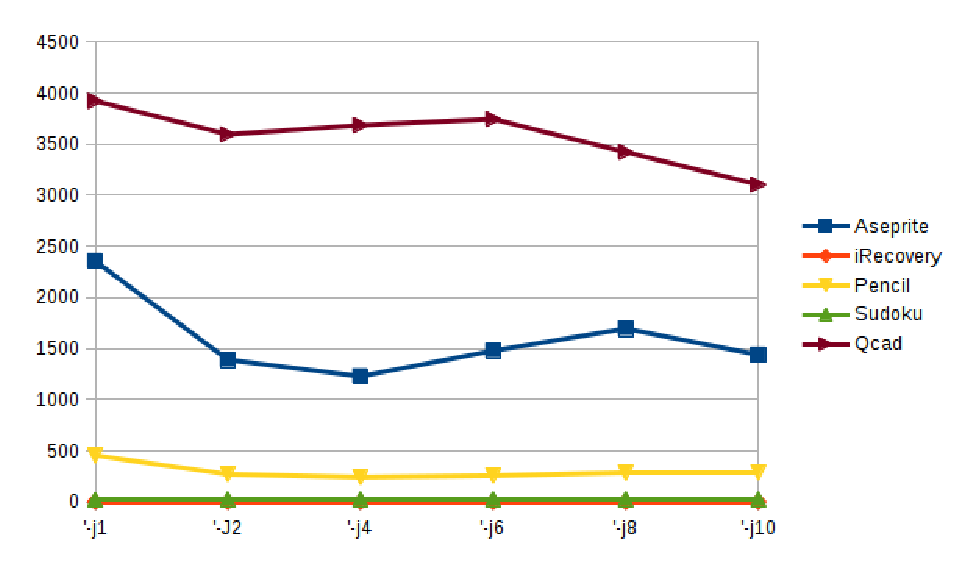
\includegraphics{figuras/graficos/linux_processamento_paralelo.eps}
            \caption{Gráfico flags de processamento paralelo no Linux}
            \label{flags_de_processamento_paralelo_linux}
        \end{figure}

        \begin{figure}[!h]
            \centering
                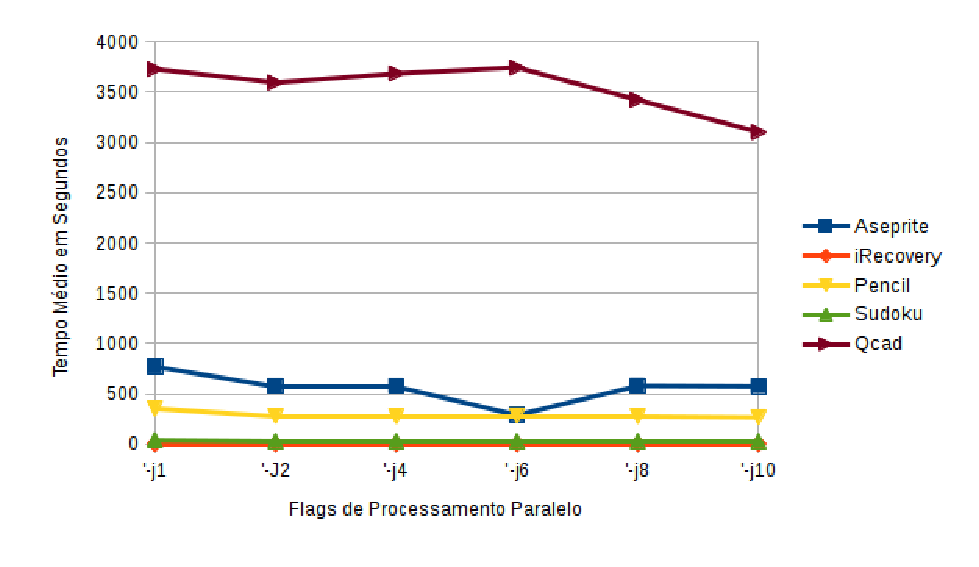
\includegraphics{figuras/graficos/mac_os_processamento_paralelo.eps}
            \caption{Gráfico flags de processamento paralelo Mac OS Yosemite}
            \label{flags_de_processamento_paralelo_mac_os}
        \end{figure}

        \begin{figure}[!h]
            \centering
                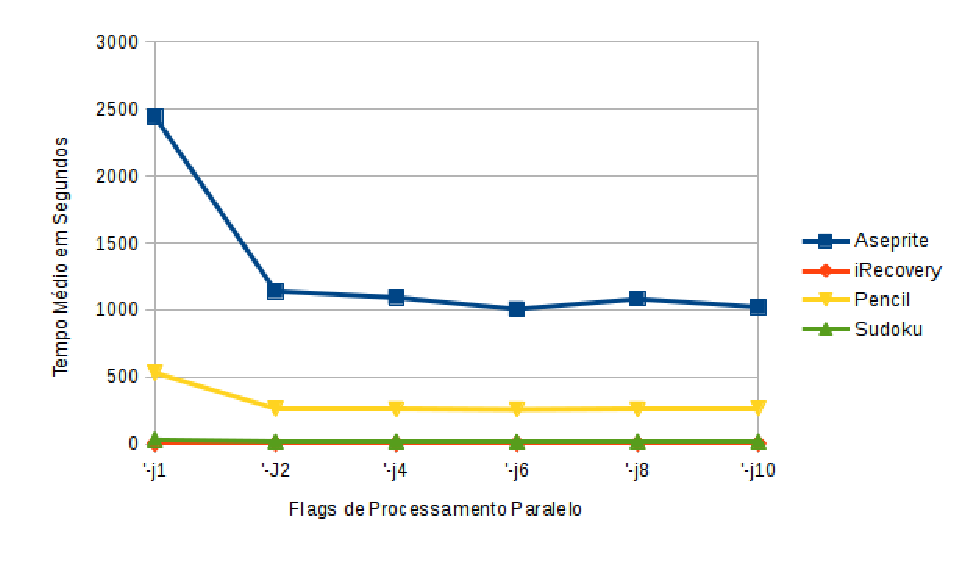
\includegraphics{figuras/graficos/windows_processamento_paralelo.eps}
            \caption{Gráfico flags de processamento paralelo no Windows 7}
            \label{flags_de_processamento_paralelo_windows}
        \end{figure}

\begin{itemize}
    \item Analise

    Com a coleta de dados e a geração dos gráficos conclue-se:
    
    \begin{enumerate}
        \item Independente do sistema operacional com a utilização da \textit{flags -j}
 o tempo de compilação mais perceptível em projetos que demoram mais de 8 minutos para compilar,
 gerando uma redução de até 50\% com 2 threads.
        \item Independente do sistema operacional não necessáriamente o aumento
 da quantidade de threads aumenta o tempo de compilação, uma vez que analisando
 como exemplo o projeto aseprite ou o qcad do \texttt{-j6} para o \texttt{-j8} o tempo de compilação
 aumenta para o projeto aseprite e reduz para o projeto qcad, e em outros
 momentos ocorre o inverso.
    \end{enumerate}
\end{itemize}

\clearpage
\subsection{Ferramentas Auxiliares}

\begin{itemize}
    \item Tabelas e Gráficos
\end{itemize}

\subsubsection*{Aseprite}
%PROJETO ASEPRITE TABELAS 

\begin{table}[!ht]
\centering
\tiny
\caption{Aseprite - Ferramentas Auxiliares no Linux}
\label{tab:ferramentas_auxliares:linux:aseprite}
\begin{tabular}{lll}
\textbf{Aseprite} & \textbf{ccache} &  \textbf{gold}  \\ \toprule
1                 &  2416.7725      &   2299.0718       \\ 
2                 &  327.7167       &   2210.9459       \\ 
3                 &  324.1109       &   2350.9201       \\ 
4                 &  328.9366       &   2308.0564       \\ 
5                 &  345.3292       &   2219.1003       \\ 
6                 &  347.0681       &   2288.3468       \\ 
7                 &  332.0379       &   2314.2384       \\ 
8                 &  329.9954       &   2280.3554       \\ 
9                 &  328.3070       &   2229.5886       \\ 
10                &  325.5209       &   2206.4399       \\ \bottomrule
Média             &  540.5795       &   2270.7064       \\ 
\end{tabular}        
\end{table}

\begin{table}[!ht]
\centering
\tiny
\caption{Aseprite - Ferramentas Auxiliares no Mac OS Yosemite}
\label{tab:ferramentas_auxliares:mac:aseprite}
\begin{tabular}{lll}
\textbf{Aseprite} & \textbf{ccache} &  \textbf{gold}  \\ \toprule
1            & 911.7870 &  -    \\ 
2            & 144.8385 &  -    \\ 
3            & 145.3597 &  -    \\ 
4            & 148.3864 &  -    \\ 
5            & 133.6848 &  -    \\ 
6            & 130.1691 &  -    \\ 
7            & 127.6144 &  -    \\ 
8            & 120.7987 &  -    \\ 
9            & 117.4732 &  -    \\ 
10           & 118.0802 &  -    \\ \bottomrule
Média        & 209.8192 &  -    \\ 
\end{tabular}
\end{table}

\begin{table}[!ht]
\centering
\tiny
\caption{Aseprite - Ferramentas Auxiliares no Windows 7}
\label{tab:ferramentas_auxliares:windows:aseprite}
\begin{tabular}{lll}
\textbf{Aseprite} & \textbf{ccache} &  \textbf{gold}  \\ \toprule
1                 & 2365.1563       &  -    \\ 
2                 & 596.2813        &  -    \\ 
3                 & 586.1250        &  -    \\ 
4                 & 605.1875        &  -    \\ 
5                 & 572.9375        &  -    \\ 
6                 & 587.1563        &  -    \\ 
7                 & 584.3125        &  -    \\ 
8                 & 571.2500        &  -    \\ 
9                 & 573.7656        &  -    \\ 
10                & 575.1094        &  -    \\ \bottomrule
Média             & 761.7281        &  -    \\ 
\end{tabular}
\end{table}

\clearpage
\subsubsection*{iRecoveryplusplus}
%PROJETO IRECOVERYPLUSPLUS TABELAS 

\begin{table}[!ht]
\centering
\tiny
\caption{iRecoveryplusplus - Ferramentas Auxiliares no Linux}
\label{tab:ferramentas_auxliares:linux:irecoveryplusplus}
\begin{tabular}{lll}
\textbf{iRecoveryplusplus} & \textbf{ccache} &  \textbf{gold}  \\ \toprule
1           & 1.1174 &  0.9923    \\ 
2           & 1.1672 &  0.9687    \\ 
3           & 1.1334 &  1.0159    \\ 
4           & 1.2546 &  1.0125    \\ 
5           & 1.1018 &  1.0264    \\ 
6           & 1.0957 &  1.0106    \\ 
7           & 1.1110 &  0.9764    \\ 
8           & 1.1503 &  0.9424    \\ 
9           & 1.1274 &  1.0066    \\ 
10          & 1.1764 &  1.0576    \\ \bottomrule
Média       & 1.1435 &  1.0009    \\ 
\end{tabular}
\end{table}

\begin{table}[!ht]
\centering
\tiny
\caption{iRecoveryplusplus - Ferramentas Auxiliares no Mac OS Yosemite}
\label{tab:ferramentas_auxliares:mac:irecoveryplusplus}
\begin{tabular}{lll}
\textbf{iRecoveryplusplus} & \textbf{ccache} &  \textbf{gold}  \\ \toprule
1      & 3.5136    &  -    \\ 
2      & 2.5199    &  -    \\ 
3      & 2.5235    &  -    \\ 
4      & 2.5468    &  -    \\ 
5      & 2.5058    &  -    \\ 
6      & 2.6408    &  -    \\ 
7      & 2.4701    &  -    \\ 
8      & 2.5113    &  -    \\ 
9      & 2.5524    &  -    \\ 
10     & 2.5642    &  -    \\ \bottomrule
Média  & 2.6348    &  -    \\ 
\end{tabular}
\end{table}

\begin{table}[!ht]
\centering
\tiny
\caption{iRecoveryplusplus - Ferramentas Auxiliares no Windows 7}
\label{tab:ferramentas_auxliares:windows:irecoveryplusplus}
\begin{tabular}{lll}
\textbf{iRecoveryplusplus} & \textbf{ccache} &  \textbf{gold}  \\ \toprule
1           & 5.1875    &  -    \\ 
2           & 4.8438    &  -    \\ 
3           & 5.3125    &  -    \\ 
4           & 5.2344    &  -    \\ 
5           & 5.0469    &  -    \\ 
6           & 5.0625    &  -    \\ 
7           & 5.2500    &  -    \\ 
8           & 4.6719    &  -    \\ 
9           & 4.6406    &  -    \\ 
10          & 5.1563    &  -    \\ \bottomrule
Média       & 5.0406    &  -    \\ 
\end{tabular}
\end{table}


\clearpage
\subsubsection*{Pencil}
%PROJETO PENCIL TABELAS 

\begin{table}[!ht]
\centering
\tiny
\caption{Pencil - Ferramentas Auxiliares no Linux}
\label{tab:ferramentas_auxliares:linux:pencil}
\begin{tabular}{lll}
\textbf{Pencil} & \textbf{ccache} &  \textbf{gold}  \\ \toprule
1          & 474.0012  &   459.5160   \\ 
2          & 137.0085  &   458.7100   \\ 
3          & 138.0875  &   457.7532   \\ 
4          & 140.2100  &   456.7455   \\ 
5          & 141.4131  &   458.2821   \\ 
6          & 139.4786  &   456.1067   \\ 
7          & 140.0177  &   458.7202   \\ 
8          & 140.1902  &   455.9186   \\ 
9          & 140.1566  &   456.5629   \\ 
10         & 140.0372  &   455.3661   \\ \bottomrule
Média      & 173.0601  &   457.3681   \\ 
\end{tabular}
\end{table}

\begin{table}[!ht]
\centering
\tiny
\caption{Pencil - Ferramentas Auxiliares no Mac OS Yosemite}
\label{tab:ferramentas_auxliares:mac:pencil}
\begin{tabular}{lll}
\textbf{Pencil} & \textbf{ccache} &  \textbf{gold}  \\ \toprule
1     & 378.6207  &  -    \\ 
2     & 74.1466   &  -    \\ 
3     & 75.3693   &  -    \\ 
4     & 73.7821   &  -    \\ 
5     & 73.5666   &  -    \\ 
6     & 73.7731   &  -    \\ 
7     & 73.3548   &  -    \\ 
8     & 73.2855   &  -    \\ 
9     & 73.8306   &  -    \\ 
10    & 74.1168   &  -    \\ \bottomrule
Média & 104.3846  &  -    \\ 
\end{tabular}
\end{table}

\begin{table}[!ht]
\centering
\tiny
\caption{Pencil - Ferramentas Auxiliares no Windows 7}
\label{tab:ferramentas_auxliares:windows:pencil}
\begin{tabular}{lll}
\textbf{Pencil} & \textbf{ccache} &  \textbf{gold}  \\ \toprule
1        & 615.7969  &  -    \\ 
2        & 135.4063  &  -    \\ 
3        & 136.8594  &  -    \\ 
4        & 134.1406  &  -    \\ 
5        & 132.4688  &  -    \\ 
6        & 131.5625  &  -    \\ 
7        & 136.4844  &  -    \\ 
8        & 132.2031  &  -    \\ 
9        & 129.3750  &  -    \\ 
10       & 132.5625  &  -    \\ \bottomrule
Média    & 181.6859  &  -    \\ 
\end{tabular}
\end{table}

\clearpage
\subsubsection*{Sudoku}
%PROJETO SUDOKU TABELAS 

\begin{table}[!ht]
\centering
\tiny
\caption{Sudoku - Ferramentas Auxiliares no Linux}
\label{tab:ferramentas_auxliares:linux:sudoku}
\begin{tabular}{lll}
\textbf{Sudoku} & \textbf{ccache} &  \textbf{gold}  \\ \toprule
1          & 23.9157 & 25.3930  \\ 
2          & 2.2334  & 20.7669  \\ 
3          & 2.1856  & 20.4777  \\ 
4          & 2.1651  & 20.8600  \\ 
5          & 2.2444  & 20.7520  \\ 
6          & 2.3041  & 20.6778  \\ 
7          & 2.2018  & 20.7493  \\ 
8          & 2.1199  & 20.6848  \\ 
9          & 2.1500  & 20.6467  \\ 
10         & 2.0455  & 20.6966  \\ \bottomrule
Média      & 4.3565  & 21.1705  \\ 
\end{tabular}
\end{table}

\begin{table}[!ht]
\centering
\tiny
\caption{Sudoku - Ferramentas Auxiliares no Mac OS Yosemite}
\label{tab:ferramentas_auxliares:mac:sudoku}
\begin{tabular}{lll}
\textbf{Sudoku} & \textbf{ccache} &  \textbf{gold}  \\ \toprule
1     &  44.0081 &  -    \\ 
2     &  3.2837  &  -    \\ 
3     &  3.2250  &  -    \\ 
4     &  3.2143  &  -    \\ 
5     &  3.1913  &  -    \\ 
6     &  3.1352  &  -    \\ 
7     &  3.1359  &  -    \\ 
8     &  3.1883  &  -    \\ 
9     &  3.2088  &  -    \\ 
10    &  3.1640  &  -    \\ \bottomrule
Média &  7.2755  &  -    \\ 
\end{tabular}
\end{table}


\begin{table}[!ht]
\centering
\tiny
\caption{Sudoku - Ferramentas Auxiliares no Windows 7}
\label{tab:ferramentas_auxliares:windows:sudoku}
\begin{tabular}{lll}
\textbf{Sudoku} & \textbf{ccache} &  \textbf{gold}  \\ \toprule
1        & 40.4219 &  -    \\ 
2        & 5.1250  &  -    \\ 
3        & 5.0156  &  -    \\ 
4        & 4.7656  &  -    \\ 
5        & 5.2031  &  -    \\ 
6        & 5.0781  &  -    \\ 
7        & 4.9688  &  -    \\ 
8        & 4.9219  &  -    \\ 
9        & 4.8281  &  -    \\ 
10       & 5.1875  &  -    \\ \bottomrule
Média    & 8.5516  &  -    \\ 
\end{tabular}
\end{table}

\clearpage
\subsubsection*{Qcad}
%PROJETO QCAD TABELAS 

\begin{table}[!ht]
\centering
\tiny
\caption{Qcad - Ferramentas Auxiliares no Linux}
\label{tab:ferramentas_auxliares:linux:qcad}
\begin{tabular}{lll}
\textbf{Qcad} & \textbf{ccache} &  \textbf{gold}  \\ \toprule
1      & 4053.0217 &   3864.8533 \\ 
2      & 1575.0124 &   3842.8008 \\ 
3      & 1575.8025 &   3844.9988 \\ 
4      & 1586.2610 &   3853.5289 \\ 
5      & 1573.3699 &   3846.0364 \\ 
6      & 1573.6939 &   3847.6719 \\ 
7      & 1571.6429 &   3841.4281 \\ 
8      & 1577.4421 &   3842.1131 \\ 
9      & 1573.8719 &   3846.6612 \\ 
10     & 1575.6482 &   3843.5791 \\ \bottomrule
Média  & 1823.5766 &   3847.3672 \\ 
\end{tabular}
\end{table}


\begin{table}[!ht]
\centering
\tiny
\caption{Qcad - Ferramentas Auxiliares no Mac OS Yosemite}
\label{tab:ferramentas_auxliares:mac:qcad}
\begin{tabular}{lll}
\textbf{Qcad} & \textbf{ccache} &  \textbf{gold}  \\ \toprule
1    & 4429.7385 &  -    \\ 
2    & 297.5427  &  -    \\ 
3    & 210.7286  &  -    \\ 
4    & 213.6511  &  -    \\ 
5    & 221.6690  &  -    \\ 
6    & 231.8735  &  -    \\ 
7    & 234.9510  &  -    \\ 
8    & 239.9830  &  -    \\ 
9    & 266.4890  &  -    \\ 
10   & 296.9332  &  -    \\ \bottomrule
Média& 664.3560  &  -    \\ 
\end{tabular}
\end{table}

        \begin{figure}[!h]
            \centering
                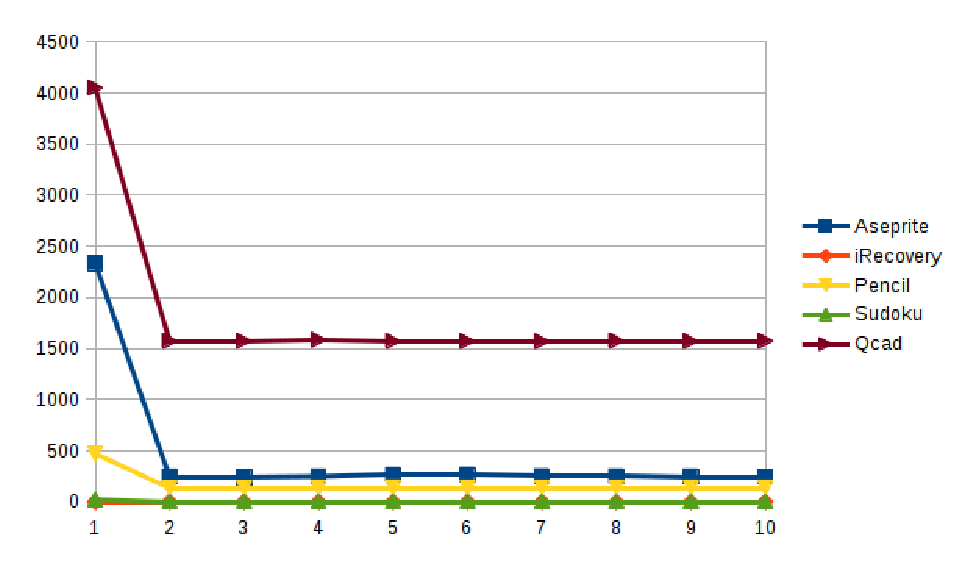
\includegraphics{figuras/graficos/linux_ccache.eps}
            \caption{Gráfico dados ferramenta ccache no Linux}
            \label{grafico_ccache_linux}
        \end{figure}

        \begin{figure}[!h]
            \centering
                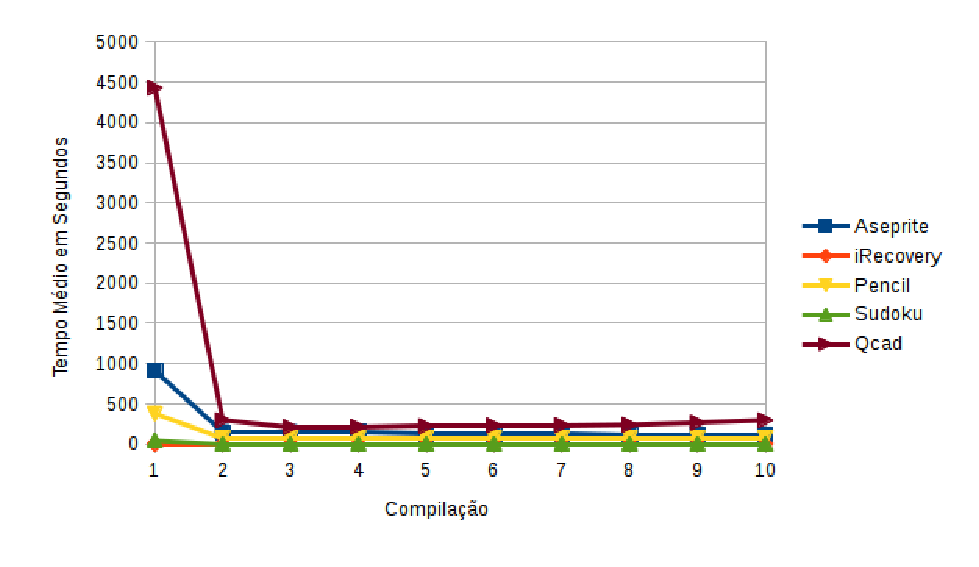
\includegraphics{figuras/graficos/mac_os_ccache.eps}
            \caption{Gráfico dados ferramenta ccache no Mac OS Yosemite}
            \label{grafico_ccache_mac_os}
        \end{figure}

        \begin{figure}[!h]
            \centering
                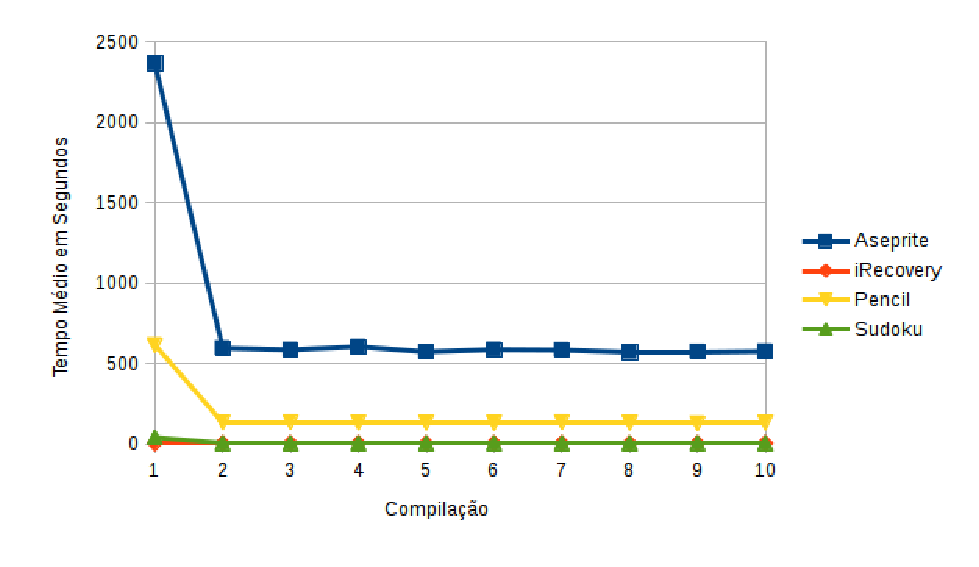
\includegraphics{figuras/graficos/windows_ccache.eps}
            \caption{Gráfico dados ferramenta ccache no Windows 7}
            \label{grafico_cache_windows}
        \end{figure}
        \begin{figure}[!h]
            \centering
                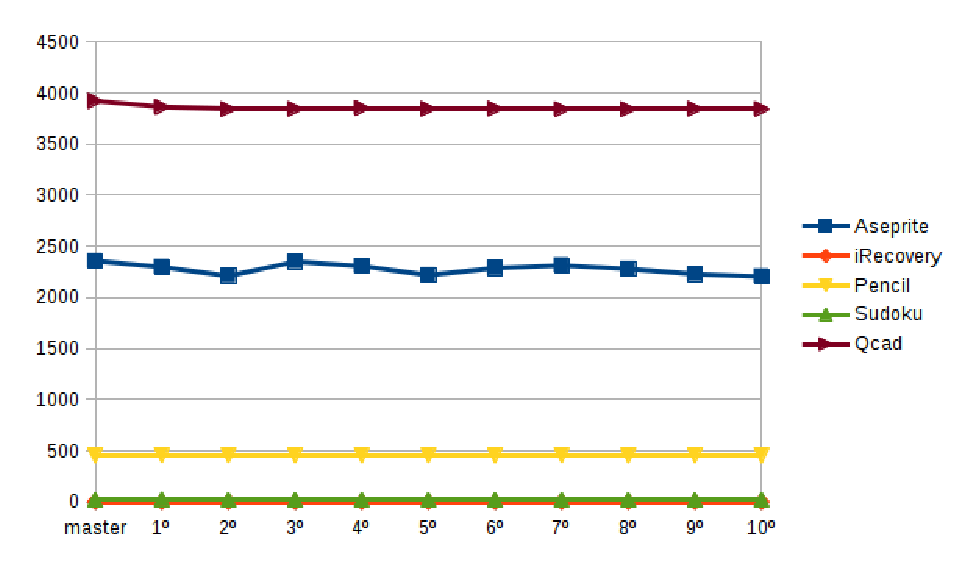
\includegraphics{figuras/graficos/linux_gold.eps}
            \caption{Gráfico dados ferramenta gold no Linux}
            \label{grafico_cache_windows}
        \end{figure}


\begin{itemize}
    \item Analise

    Com os dados coletados e os gráficos gerados conclue-se:

    \begin{enumerate}
        \item Em todos os sistemas operacionais todos os projetos
 analisados sofrerão redução de mais de 65\%  depois da primeira compilação.
        \item Analisando os gráficos em todos os ambientes o primeiro
 caso na compilação utilizando a ferramenta \textit{ccache} o tempo de compilação é o maior,
 devido a efetivar uma compilação completa do projeto, nos demais casos o tempo de compilação
 é reduzido drasticamente pois a ferramenta utiliza um sistema de cache dos arquivos, assim ao
 verificar que um arquivo já foi compilado ele não compila novamente e apenas utiliza o que foi
 compilado na primeira vez.
        \item Com a utilização da ferramenta \textit{gold} o tempo de compilação
 dos projetos ocorre uma redução pouco significativa, que obteve no maximo 12\% de
 redução do tempo de compilação dos projetos. 
        \item A utilização da ferramenta \textit{gold} teve maior impacto no projeto aseprite, que utiliza
 como gerador de makefile o cmake.
    \end{enumerate}
\end{itemize}

\clearpage
\subsection{Analise Geral}
    Com a analise de todos os dados coletados conclue-se que dependendo do sistema operacional o
 tempo de compilação dos projetos é alterado, sendo que o tempo é maior para o sistema operacional Windows 7,
 devido ao mesmo ser compilado utilizando um ambiente de desenvolvimento virtual.

    Para o sistema operacional Mac OS Yosemite os menores tempos de compilação foram encontrados neste
 sistema operacional uma vez que este utiliza como backend um conjunto de codigo modularizado e reutilizavel
 que proporcional maior performace, que é proposto pelo LLVM.

    Métodos que realizam alteração de código utilizando  não tiveram impactos relevantes, pois as alterações
 reduziram no maximo 12\% do tempo de compilação.

    Para a alteração de flags no processo de compilação a flags \texttt{-Ofast} foi a mais eficiente,
 no entanto foi póssivel visualizar este resultado apenas no projeto Aseprite, que possui o
 \textit{cmake} gerador de \textit{makefile},todos os outros projetos que utilizam o qmake
 como gerador de makefile foram ineficientes.

    No processo de compilação utilizando threads os resultados são bons uma vez que
 ao utilizar 2 \textit{threads}, o tempo de compilação foi reduzido pela métade.

    Na analise das ferramentas o \textit{gold} não foi póssivel identificar nenhuma redução significativa,
 no entanto a ferramenta \textit{ccache} a redução é significativa pois na primeira compilação o tempo o máximo
 e na segunda em diante o tempo é reduzido em mais 65\%.
